\documentclass[11pt]{article}
% Shared preamble. Deliberately built on stock `article` + widely-packaged dependencies rather than
% a venue .cls: the source has to compile for a reader who just cloned the repository, and swapping
% in acmart/neurips at submission time is a one-line change.

\usepackage[T1]{fontenc}
\usepackage[utf8]{inputenc}
\usepackage{lmodern}
\usepackage{microtype}
\usepackage[margin=1in]{geometry}
\usepackage{amsmath,amssymb}
\usepackage{booktabs}
\usepackage{array}
\usepackage{longtable}
\usepackage{graphicx}
\usepackage{xcolor}
\usepackage{caption}
\usepackage{subcaption}
\usepackage{listings}
\usepackage{enumitem}
\usepackage[hidelinks]{hyperref}
\usepackage[capitalise,noabbrev]{cleveref}
\usepackage{natbib}

\definecolor{codebg}{HTML}{F6F8FA}
\definecolor{rule}{HTML}{D0D7DE}
\definecolor{accent}{HTML}{1F4E79}

\captionsetup{font=small,labelfont=bf}
\setlist{itemsep=2pt,topsep=3pt,parsep=0pt}

\lstdefinestyle{policy}{
  basicstyle=\ttfamily\small,
  backgroundcolor=\color{codebg},
  frame=single,
  rulecolor=\color{rule},
  framesep=5pt,
  xleftmargin=6pt,
  breaklines=true,
  columns=fullflexible,
  keepspaces=true,
  showstringspaces=false,
}
\lstset{style=policy}

% Notation used throughout.
\newcommand{\Lpost}{\ensuremath{L^{\mathrm{post}}}}
\newcommand{\Rreg}{\ensuremath{\mathcal{R}}}
\newcommand{\headroom}{\ensuremath{H}}
\newcommand{\policyfam}{\ensuremath{\Theta}}
\newcommand{\shockstep}{\ensuremath{t^{\star}}}

% Data-dependent prose. Defaults say "pending" out loud, so a draft compiled before the sweep
% finishes announces that on the page instead of quietly reading as finished; the generated file
% \renewcommand's them once numbers exist.
\newcommand{\ResultsAbstractSentence}{\textcolor{red}{[results sentence pending the completed sweep]}}
\newcommand{\ResultsBody}{\textcolor{red}{[Results section pending the completed sweep. The tables
below are generated from the analysis artifact and are empty until it exists.]}}

% A boxed remark for the claims a reviewer will want to find quickly.
\newenvironment{takeaway}
  {\par\smallskip\noindent\begin{tabular}{@{}p{0.965\linewidth}@{}}\toprule\itshape}
  {\\\bottomrule\end{tabular}\par\smallskip}

% Fallbacks FIRST, so the generated files below can \renewcommand them. The other order looks
% harmless and is not: the generated file loads before the fallback exists, \renewcommand errors on
% an undefined command, and LaTeX carries on — leaving the fallback's "?" in the shipped PDF while
% the build reports only a warning. That is exactly what happened to \MDEFraction, which printed as
% "worth roughly ?%" in a compiled draft.
\providecommand{\FrozenCost}{?}\providecommand{\BestFixedCost}{?}
\providecommand{\SwitchCost}{?}\providecommand{\DivergenceSeed}{?}
\providecommand{\MDEFraction}{?}\providecommand{\MDEWorst}{?}\providecommand{\MDEMemory}{?}
% Overrides the "pending" defaults once scripts/make_tables.py has real numbers to state.
\newcommand{\FreshnessGateRef}{(\cref{sec:ctx-outcome})}
\IfFileExists{generated/results_prose.tex}{% not enough results yet; the preamble's pending defaults stand.
}{}
\IfFileExists{generated/divergence_facts.tex}{% GENERATED by scripts/make_figures.py — do not edit.
\newcommand{\FrozenCost}{173.7}
\newcommand{\BestFixedCost}{170.0}
\newcommand{\SwitchCost}{123.5}
\newcommand{\DivergenceSeed}{0}
}{}
\IfFileExists{generated/library_facts.tex}{\newcommand{\libWorlds}{6}
\newcommand{\libRows}{10}
\newcommand{\libDefined}{5}
\newcommand{\libFracRows}{3/9}
\newcommand{\libFracBest}{3/5}
\newcommand{\libFracMedian}{2/5}
\newcommand{\libMaxAdapt}{1.359}
\newcommand{\libMaxRecovered}{26}
\newcommand{\libEpiMin}{1.000}
\newcommand{\libEpiMax}{1.199}
\newcommand{\libEpiConfigs}{5}
\newcommand{\libBestWorld}{monetary}
\newcommand{\libBestAdapt}{1.359}
\newcommand{\libBestStale}{1.560}
}{}
\IfFileExists{generated/lockin_facts.tex}{\newcommand{\lockinOnsetOwn}{0.40}
\newcommand{\lockinOnsetBare}{1.00}
\newcommand{\lockinOnsetForeign}{1.00}
\newcommand{\lockinBreak}{10}
\newcommand{\lockinBarePre}{0.84}
\newcommand{\lockinBarePost}{0.83}
\newcommand{\lockinOwnPre}{0.04}
\newcommand{\lockinOwnPost}{0.10}
\newcommand{\lockinForeignPre}{0.44}
\newcommand{\lockinForeignPost}{0.84}
\newcommand{\lockinBareDelta}{-0.01}
\newcommand{\lockinOwnDelta}{+0.06}
\newcommand{\lockinForeignDelta}{+0.40}
\newcommand{\lockinBareP}{0.906}
\newcommand{\lockinOwnP}{0.280}
\newcommand{\lockinForeignP}{0.018}
}{}

\title{\bfseries When Does Adaptation Have Room to Matter?\\
\large Measuring adaptation headroom, and attributing it to harness components,\\
for language-model controllers that govern through executable policy code}

\author{}
\date{}

\begin{document}
\maketitle

\begin{abstract}
\noindent
Language-model agents are increasingly proposed as policy-makers for simulated societies and
economies, and a fast-growing literature asks whether the surrounding \emph{harness}---the code that
decides what the model is shown and remembers---can be optimized or evolved. Both literatures share
a blind spot: they report whether an agent adapted without first establishing whether the
environment left any room to adapt \emph{into}. We make that quantity computable. For a structural
break, we calibrate three references inside one shared policy vocabulary---the rule that was optimal
before the break and held fixed, the best \emph{fixed} rule over the whole broken horizon chosen in
hindsight, and the best clairvoyant \emph{switch}---and show that what a stale rule costs factors
exactly into an \emph{adaptation headroom} and a \emph{robustness headroom}. Only the first is
recoverable by an agent that notices and revises; the second was available to anyone who wrote a
better rule in the first place.

The distinction is not decorative. In two of the four regimes we calibrate, a stale rule costs
$18$--$44\%$ while adaptation headroom is $1.00$--$1.01$: the optimum never moved, so an agent
evaluated there would look rigid while facing no adaptive problem, and would be prescribed
responsiveness for something responsiveness cannot touch. Measuring first also tells us which shocks
are worth studying at all: feedback rules \emph{absorb} shocks to the state they observe---prevalence
rises, the rule fires more often---and cannot absorb shocks to their own \emph{instrument}, where the
observable no longer says what the lever is worth. Adaptation headroom turns out to be a narrow band
in both severity and price, and it is not monotone in either.

On that regime we place a regent that governs by emitting sandboxed executable Python policy---not
a scalar, not a schema-bound JSON object---and specify a pre-registered $2^3$ factorial over three
harness channels (failure trace, realized-outcome feedback, episodic memory) at a matched
language-model call budget on $20$ paired seeds. Coverage of that design is reported as a generated
fact rather than asserted (\cref{sec:results}).
\ResultsAbstractSentence
The harmful channel is episodic memory, and it is harmful in a specific way: it does not misinform
the regent, it stops it revising, collapsing the rate at which the enacted law changes from $0.85$ to
$0.08$. Three pre-registered repairs to how precedent is presented all failed. A fourth arm replaces
the regent's own episodes with a different regent's, holding the retrieval rule, ranking, phrasing
and episode count fixed, and recovers most of the lost revision ($0.63$) while removing the entire
loss penalty. The mechanism is not that the regent recognises the precedent as somebody else's---the
prompt attributes the donor's decisions to the regent either way---but that precedent drawn from
one's \emph{own} trajectory is retrieved from $2.4\times$ nearer the current situation. In a world
that recurs, similarity-ranked recall of one's own history returns something close to a copy of the
last decision, and a near-copy is repeated. That makes the load-bearing design choice the
\emph{retrieval rule}, not the existence of the memory.
We release the environment, the calibration procedure, the pre-registration, and the recorded
model-call tapes that make every run replayable without an API key.
\end{abstract}

% The one sentence of the abstract that depends on data. Defined here so a draft compiled before
% the sweep finishes says so, rather than quietly asserting a number nobody measured.
\providecommand{\ResultsAbstractSentence}{\textcolor{red}{[results sentence pending the completed
sweep]}}

\section{Introduction}

A recurring proposal in computational social science is to put a language model in the seat of a
governing authority---setting tax rates \citep{wang2025taxagent}, running a macroeconomy
\citep{li2023econagent}, or managing a commons \citep{piatti2024govsim}---and to ask whether it
governs well. A parallel and much faster-moving literature asks a different question about the same
systems: how much of an agent's competence lives not in the model but in the \emph{harness} around
it, the code deciding what to store, retrieve, and present
\citep{lee2026metaharness,chen2026agentspec,ning2026codeasharness}, and whether that harness can
itself be searched or evolved \citep{hu2024adas,zhang2024aflow,zhang2025dgm}.

Both literatures are, right now, being asked hard questions about their evidence.
\citet{wang2026rethinking} report that automatic harness evolution does not reliably beat
budget-matched test-time scaling and generalizes poorly, in part because it is evaluated on the same
benchmark used to search. \citet{chen2026agentspec} find that scaffold performance is governed by component compatibility
and \emph{interaction} rather than by isolated module strength; if that holds here, the
one-at-a-time ablations most papers report cannot be read as component values. And across LLM social
simulation, \citet{ye2026trails} show a simulation's cooperation rate moving by up to $76$
percentage points under an unaudited change to persona format and game-instruction framing.

We think a more basic problem sits underneath these. Studies of adaptation to a changing world
report the adapting agent's performance against a non-adapting baseline, and treat the difference as
the effect. But that difference is bounded above by a property of the environment that is almost
never reported: how much better \emph{anything} could have done by adapting. If a shock leaves a
fixed rule near-optimal, then a null result says nothing about the agent; if a shock makes every
policy diverge, the comparison is between two collapses. Neither is a finding about governance, and
from the outside the two are indistinguishable from a genuine null.

\paragraph{Contributions.}
\begin{enumerate}[leftmargin=1.4em]
\item \textbf{A measurement that prices a distinction control theory already draws}
(\cref{sec:headroom,sec:decomposition}). Fault-tolerant control has long separated \emph{passive}
schemes, which hold one fixed controller made robust to a presumed fault class, from \emph{active}
ones, which detect the fault and reconfigure \citep{zhang2008reconfigurable}; that the choice between
them depends on the fault set, rather than one dominating, is the field's own conclusion
\citep{jiang2012comparative}. We do not claim the distinction. We claim a way to \emph{price} it
before committing to either, in a setting where the controller is an institution and the fault is a
policy instrument losing efficacy. Three references calibrated in one shared vocabulary---the
pre-break optimum held fixed, the best \emph{fixed} rule in hindsight, and the best clairvoyant
\emph{switch}---factor staleness exactly into a robustness headroom (what the best passive scheme
recovers) and an adaptation headroom (what only reconfiguration recovers), and place any controller
on a normalized scale between the last two. The factorization is exact and multiplicative, so the two
cannot be traded off rhetorically. Because it is computed before any agent runs, it also makes the
severity of a designed shock an auditable choice rather than a researcher degree of freedom.

What is genuinely new is the empirical answer in this domain, and it is the uncomfortable one: the
active term---the entire justification for building adaptive institutions---is the smaller of the two
almost everywhere we look, and in some worlds is exactly zero while the passive term is large. An
authority evaluated there registers as rigid while facing no adaptive problem at all.

\item \textbf{Two components whose value reverses between environments}
(\cref{sec:crossworld}). Running the same factorial in a second world, \emph{both} channels that do
anything at all flip sign: episodic memory costs $1.11$ loss units in one world and recovers $371$ in
the other, and realized-outcome feedback recovers $975$ on $20/20$ seeds where elsewhere it harms.
All four contrasts are significant, and the memory pair is uncontaminated---those arms produce an
action on every decision in both worlds. A component's value is therefore not a property of the
component but of the match between what it does and what the world's failure mode requires. That
supplies a mechanism for the reported poor generalization of automatically evolved harnesses. We do
\emph{not} claim to predict the sign in advance: with two worlds we can describe what separates them,
not validate a predictor.

\item \textbf{A structural result about which shocks are worth studying}
(\cref{sec:which-shocks,sec:library}). Measuring across ten worlds with unrelated mechanics---a
monetary economy, an opinion polity, a fishery, a supply chain, a stock-flow-consistent fiscal
economy and five epidemic configurations---we find that feedback policies absorb shocks to the state
dynamics, so those regimes are near-null by construction, but cannot absorb shocks to instrument
efficacy. Adaptation headroom is a narrow band in both the severity of the break and the price of
intervention, and non-monotone in each. It is also \emph{bounded}: the largest adaptation headroom
anywhere in the library is $\libMaxAdapt\times$, so even a clairvoyant re-legislator recovers at most
$\libMaxRecovered\%$ of the incumbent rule's cost. We deliberately do not report what share of worlds
has headroom---we chose the library's contents, so no such share estimates anything, and the number
moves from $\libFracRows$ to $\libFracBest$ depending on whether one counts rows or distinct worlds
(\cref{tab:library}). We report the near-null worlds rather than discarding them, and retain two
as declared negative controls---including the one that settles the shock family our own taxonomy had
never measured.

\item \textbf{Governance by executable policy code, in a domain where the code is the point}
(\cref{sec:regent}). Existing LLM-as-authority systems emit scalars or fixed-schema objects. Our
regent emits a sandboxed Python expression that the environment re-evaluates every step, so the
enacted policy is a legible artifact---which is also a direct answer to the auditability objection
that \citet{zhong2026separating} raise against putting a language model in the control path at all.

\item \textbf{Factorial harness attribution across a structural break, at matched budget}
(\cref{sec:design,sec:results}). The design is a full $2^3$ over three \emph{different kinds} of
information; it estimates interactions rather than assuming them away, corrects across the family,
and matches the model-call budget across arms---the three things the harness literature is currently
being told it does not do.

\item \textbf{Five validity gates for scaffold ablations, every one of which this study failed
before it passed} (\cref{sec:ctx-outcome,sec:responsiveness}). Output truncation correlated with the
treatment; information channels that fired but carried no signal; reference anchors superseded by a
recalibration; a clairvoyant reference that a fixed policy could beat; and---the failure the other
four cannot see---a model that reads none of what the harness gives it, measured at $400/400$
identical decisions under a live memory channel. A sixth failure mode turned out to be a result in
its own right (\cref{sec:collapse}): one channel drives the model into unbounded deliberation on
$4$--$8\%$ of decisions while the others never exceed $0.2\%$, so a scaffold component can degrade
an agent without supplying it a single false statement. Each produced a clean, plausible, wrong number that
no amount of care in the writing would have caught, and each is now an automatic check that refuses
to let the tables be read. A literature being asked for better evidence
needs transferable failure modes at least as much as it needs another effect.
\end{enumerate}

\section{Related work}
\label{sec:related}

\paragraph{Harnesses as an object of study.}
The lineage from prompt- and pipeline-level optimization
\citep{yang2023opro,fernando2023promptbreeder,khattab2023dspy,yuksekgonul2024textgrad} to explicit
search over agent architectures \citep{hu2024adas,zhang2024aflow,zhang2025dgm} now has an explicit
harness-optimization branch: \citet{lee2026metaharness} search over harness \emph{source code};
\citet{chen2026agentspec} type and recombine scaffold components under controlled composition;
\citet{xu2026lifeharness} transfer a harness across models; \citet{kim2026interplay} pair harness
design with environment shift. We claim no novelty for the idea that the harness is worth studying,
nor for the term \emph{meta-harness}, which \citet{lee2026metaharness} introduced. Our contribution
is orthogonal: a way to know, in advance, whether a given environment can measure a harness
difference at all, and an application to a shock type that literature has not isolated.

One structural feature of that lineage is worth naming, because our result bears on it directly.
These systems search over designs and evaluate them on the same benchmark the search consumed:
\citet{zhang2025dgm} searches and scores on SWE-bench and Polyglot, and it is precisely this
arrangement that \citet{wang2026rethinking} identify as making reported gains hard to attribute. The
usual worry is overfitting---a harness tuned to a task set carries less to held-out tasks in the same
set. Our cross-world measurement (\cref{sec:crossworld}) suggests the sharper version: a component
selected where one failure mode dominates can be \emph{negatively} valued where another does, so a
search that never leaves its benchmark cannot see the sign of what it is optimizing, let alone its
magnitude.

\paragraph{Code as policy.}
Emitting executable code as the action is established in robotics
\citep{liang2022codeaspolicies}, reward design \citep{ma2023eureka}, and algorithm discovery
\citep{novikov2025alphaevolve}. Closest to us, \citet{guo2026codeevolution} synthesize control
policies by LLM-driven evolutionary search and argue for their inspectability; they name no concrete
control domain and do not treat non-stationarity. \citet{bosio2025combining} report the relevant
caution: language models are poor at separating program \emph{structure} from numeric
\emph{parameters}, so a code-emitting controller may be doing constant-tuning in disguise. We test
that directly by widening our reference family until it contains the functional form the regent
discovered (\cref{sec:wide-oracle}).

\paragraph{LLM authorities and the auditability objection.}
\citet{wang2025taxagent} have an LLM set tax rates; \citet{li2023econagent} drive macroeconomic
agents; \citet{piatti2024govsim} study commons governance. In each the action is a number or a
fixed-schema record. Against this, \citet{zhong2026separating} argue for confining the LLM to
\emph{diagnosis} and leaving control to deterministic formulas, reporting both an accuracy advantage
and a traceability one. Policy-as-code is a substantive reply---the enacted rule is a short, readable
expression that can be diffed and archived---but only if inspectability is measured rather than
asserted, which is why we report the enacted policies themselves alongside the losses.

\paragraph{Adaptation after a structural break.}
That a policy rule's own effect changes when the regime changes is the Lucas critique
\citep{lucas1976critique}, and that a measure targeted by policy ceases to be a good measure is
Goodhart's \citep{goodhart1984monetary}. The nearest empirical neighbor is
\citet{decurto2026narratives}, who compare adaptive against frozen policy under a mid-simulation
structural perturbation with paired seeds and effect sizes; their agent emits a five-field
parameterized object rather than code, and, like the non-stationary in-context RL literature
\citep{run2026icrlsurvey}, they report the adaptive-versus-frozen gap without bounding it from above.

\paragraph{Methodological norms.}
We adopt the emerging reproducibility expectations for LLM social simulation
\citep{sarangi2026ease,ye2026trails,luo2026preconditions,li2026policypractice}: a pre-registered
primary metric, paired seeds, released code and configuration, and---because the decisive actor is a
sampled model---a recorded call tape that replays every reported run byte-for-byte without a key.

\section{Governance as control under a structural break}
\label{sec:setting}

A \emph{world} is a discrete-time stochastic system with state $x_t$, evolving under parameters
$\phi_t$ and a control $u_t$ supplied by an \emph{institution}. At each decision step the regent
observes a partial view $o_t$ and installs a control law $\pi$; the world re-evaluates
$u_t = \mathrm{clip}(\pi(o_t))$ at \emph{every} step, not only at decision steps, so an institution
is a standing rule rather than a sequence of one-off interventions. This is the distinction between
governing and micromanaging, and it is what makes the emitted policy an object with content.

A \emph{structural break} at $\shockstep$ replaces $\phi_{\shockstep}$ with $\phi'$ without
announcement. Nothing in $o_t$ names the break; the regent can only infer it from the divergence
between what its policy used to achieve and what it now achieves. We score the post-break window,
\begin{equation}
\Lpost(\pi) \;=\; \frac{1}{T-\shockstep}\sum_{t=\shockstep}^{T}\ell\bigl(x_t, u_t\bigr),
\end{equation}
because the pre-break window is one where a pre-break-optimal rule is optimal by definition, and
averaging it in dilutes---and at plausible parameter settings inverts---the comparison.

\section{Adaptation headroom}
\label{sec:headroom}

Fix a policy family $\policyfam$: a functional form together with the grid its parameters range
over. Define
\begin{align}
\pi_{\mathrm{frozen}} &= \arg\min_{\pi \in \policyfam} \; L_{\mathrm{pre}}(\pi),
&\pi_{\mathrm{oracle}} &= \arg\min_{\pi \in \policyfam} \; \Lpost(\pi),
\end{align}
where $L_{\mathrm{pre}}$ is the loss on the stationary pre-break world and $\Lpost$ is the
post-break loss on the world that actually breaks. The two differ in exactly one respect: when they
were allowed to look. Both are then scored on the same broken world over the same seeds, giving
\begin{equation}
\headroom \;=\; \frac{\Lpost(\pi_{\mathrm{frozen}})}{\Lpost(\pi_{\mathrm{oracle}})},
\qquad
\Rreg(\pi) \;=\;
\frac{\Lpost(\pi) - \Lpost(\pi_{\mathrm{oracle}})}
     {\Lpost(\pi_{\mathrm{frozen}}) - \Lpost(\pi_{\mathrm{oracle}})}.
\end{equation}

\subsection{The decomposition: costly is not the same as un-adaptive}
\label{sec:decomposition}

A single ratio is not enough, and the reason matters. Let $\pi_{\mathrm{fixed}}$ be the best
\emph{fixed} law over the whole broken horizon chosen in hindsight, and $\pi_{\mathrm{switch}}$ the
best (pre-leg, post-leg) pair. Then
\begin{equation}
\underbrace{\frac{L(\pi_{\mathrm{frozen}})}{L(\pi_{\mathrm{switch}})}}_{\text{staleness}}
\;=\;
\underbrace{\frac{L(\pi_{\mathrm{fixed}})}{L(\pi_{\mathrm{switch}})}}_{\text{adaptation headroom}}
\;\times\;
\underbrace{\frac{L(\pi_{\mathrm{frozen}})}{L(\pi_{\mathrm{fixed}})}}_{\text{robustness headroom}} .
\end{equation}

Staleness is what studies of institutional rigidity report: how much worse the old rule is after the
break. It answers no design question on its own, because it conflates two remedies. The adaptation
term is recoverable \emph{only} by changing behaviour mid-run. The robustness term is recoverable by
having legislated a different standing rule at the outset, with no adaptation whatsoever.

The two come apart completely, and \cref{tab:headroom} shows they do so along both axes we can vary.
Holding the price of intervention fixed and driving the instrument to \emph{total} failure gives a
staleness cost of $1.18\times$ with an adaptation headroom of $1.01\times$; holding the break fixed
and raising the price instead gives $1.44\times$ staleness with adaptation of exactly $1.00\times$.
In both, the best standing rule chosen in hindsight is as good as the best clairvoyant switch, so
the entire cost is a rule-design failure. An agent evaluated in either cell would appear rigid while
facing no adaptive problem at all, and would be prescribed the wrong reform---greater
responsiveness, faster review cycles, better monitoring---for a problem that responsiveness cannot
touch.

The direction is worth stating because it is not the intuitive one, and it was not ours: the harsher
cell was added on the assumption that a bigger break leaves more for adaptation to recover. Past a
point the failure is complete enough that a single robust rule dominates, and responsiveness buys
nothing. \textbf{Adaptation headroom is a narrow band in both severity and price}, and the flagship
regime is the only cell of the four we measured that sits inside it.

Our first version of this comparison varied severity and price \emph{together}, which would have
attributed the whole effect to severity. Separating them is what turned a striking observation into
a controlled one; we report the confounded version and its correction in the deviation log rather
than only the conclusion.

We take the practical implication seriously: \emph{a costly rule and a rule that must change are
different diagnoses, and only the second is a case for a more attentive government.}

\medskip
$\Rreg = 0$ is clairvoyant and $\Rreg = 1$ is ``did no better than never adapting''. We do not clip
$\Rreg$. Values below $0$ are possible and informative, because the oracle is optimal only
\emph{within} $\policyfam$ while a code-emitting regent is not confined to it; values above $1$ mean
the controller did actively worse than leaving the old rule alone, which is the failure mode a
governance paper most needs to be able to report.

Three properties make this worth the compute it costs. It is computed \emph{before} any agent runs,
so the severity of a designed shock stops being a free parameter tuned until the result appears. It
is unitless, so epidemic burden and control-effort loss land on one scale. And it fails loudly:
when $\pi_{\mathrm{frozen}} = \pi_{\mathrm{oracle}}$, the shock provably does not move the optimum,
and no experiment in that regime can say anything about adaptation.

\begin{takeaway}
An adaptation result without a headroom measurement is unfalsifiable in one direction: a null cannot
be distinguished from an environment in which no effect was available.
\end{takeaway}

\subsection{Two calibration traps}
\label{sec:traps}

Both of the following produced clean, plausible, and wrong numbers in our own first pass, and we
report them because they are easy to repeat.

\emph{Calibrating on a component instead of the objective.} Optimizing a reference for mean squared
error, or for cumulative infections, while the objective also prices control effort or lockdown
cost, drives every reference to a corner of the grid---use the maximum lever always. Corner optima
are regime-invariant, so every environment we tested reported $\headroom \approx 1.0$. That was an
artifact of the calibration metric, not a property of the worlds.

\emph{Letting an empty post-shock window score zero.} If a run can terminate before $\shockstep$,
then a policy that ends the episode early has an empty post-shock window, and a mean over no rows is
$0$---a perfect score. In the epidemic model this made ``let it burn out'' the optimal post-shock
policy. We score an empty window as $+\infty$ and, more fundamentally, make the disease endemic so
that it cannot be outlasted.

\emph{Scoring only the post-break window, which rewards passivity.} This one we pre-registered and
had to withdraw. A policy that never intervenes is wrong before the break and, precisely because the
break disables the instrument, close to right after it---so it scores well on a post-window metric
without having adapted to anything. The no-harness control arm made this visible by reaching
$\Rreg \approx 0.11$ while emitting $64\%$ bare constants. Scoring the full horizon against the best
\emph{fixed} law in hindsight removes the free lunch, because no fixed law is optimal on both sides
of a break that moves the optimum. The deviation is logged in full rather than quietly folded in.

\emph{Composing the clairvoyant reference from separately-optimal legs.} The natural construction of
the switching reference---take the law that is best on a stationary pre-break world, then the law
that is best on the post-break window---is wrong whenever the state carries information across the
break, which in a compartmental model it always does: the pre-break leg decides how much of the
population is still susceptible when the break lands. The error is not subtle in its consequences.
In our harsher severity cell the composed reference scored \emph{worse} than the best fixed law
($\headroom = 0.92$), which is impossible for a genuine upper bound, since switching subsumes not
switching. We now search the $(\text{pre}, \text{post})$ pair jointly over a shortlist of pre-legs,
and treat $\headroom < 1$ as a hard signal that the reference search is under-powered rather than as
a finding. This check is worth building in: a reference that can be beaten by a special case of
itself is detectable automatically, and a normalized regret computed against one is meaningless in a
way no amount of careful statistics downstream would reveal.

\section{Which shocks leave room to adapt}
\label{sec:which-shocks}

\begin{table}[t]\centering\small
\caption{\textbf{Decomposing what a stale rule costs.} All references are calibrated by
exhaustive search over the same policy vocabulary, on the same broken world, over the same seeds;
they differ only in what they were allowed to know. \emph{staleness}
$=L_{\text{frozen}}/L_{\text{switch}}$ is what the pre-break-optimal rule costs after the
break---the quantity a study of institutional rigidity usually reports, and on its own ambiguous.
It factors into \emph{adaptation headroom} $=L_{\text{fixed}}/L_{\text{switch}}$, the
part recoverable \emph{only} by changing behaviour mid-run, and \emph{robustness headroom}
$=L_{\text{frozen}}/L_{\text{fixed}}$, the part recoverable by having legislated a better
standing rule in the first place. The severe regime is the instructive case: a large staleness cost
with \emph{no} adaptation headroom at all. There the polity needed a better rule, not a more
attentive government---and reporting staleness alone would have called it an adaptation failure and
prescribed the wrong remedy.}
\label{tab:headroom}
\begin{tabular}{@{}l r r r r r r@{}}
\toprule
& \multicolumn{3}{c}{full-horizon loss} & \multicolumn{3}{c}{decomposition} \\
\cmidrule(lr){2-4} \cmidrule(lr){5-7}
regime & frozen & best fixed & switching & staleness & \textbf{adaptation} & robustness \\
\midrule
epidemic & 27.972 & 25.229 & 21.267 & 1.315 & \textbf{1.186} & 1.109 \\
epidemic\_pricey & 39.037 & 27.125 & 27.125 & 1.439 & \textbf{1.000} & 1.439 \\
epidemic\_severe & 29.967 & 25.648 & 25.482 & 1.176 & \textbf{1.007} & 1.168 \\
scalar & 0.036 & 0.033 & 0.032 & 1.125 & \textbf{1.039} & 1.083 \\
\bottomrule
\end{tabular}
\end{table}


\begin{figure}[t]\centering
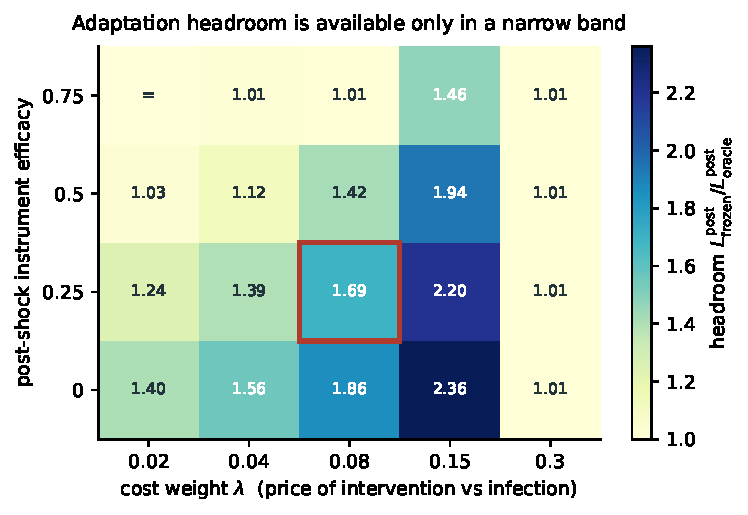
\includegraphics[width=0.82\linewidth]{generated/fig_headroom_surface}
\caption{\textbf{Headroom over the cost weight $\lambda$ and post-break instrument efficacy.}
Cells marked ``='' are ones where the calibrated pre- and post-break policies are \emph{identical}:
the break provably does not move the optimum, so nothing can be learned there. The band is bounded
on both sides and for the same reason---at $\lambda \le 0.02$ permanent maximal lockdown is optimal
and at $\lambda = 0.3$ doing nothing is, and a corner optimum is invariant to the regime. Only
$6/20$ cells combine a moved optimum with $\headroom \ge 1.5$. The red box is the pre-registered
operating point; note that it is inside the usable band rather than at its maximum, which is
deliberate---selecting the cell that maximizes the effect is the researcher degree of freedom this
measurement exists to remove.}
\label{fig:surface}
\end{figure}

The pattern in \cref{tab:headroom,fig:surface} has a mechanical explanation. A policy of the form ``intervene
when the observable exceeds $\theta$'' is feedback. When a shock raises the state's magnitude---a
more transmissible pathogen, a less stable plant---the rule fires more often on its own, and remains
close to optimal without anyone changing it. The observable still means what it meant.

An \emph{instrument} shock breaks that. When the lever's efficacy falls while its price does not, no
threshold on the observable recovers the right behaviour, because the mapping from observation to
correct action has changed rather than the observation. The rule keeps paying full price for a
fraction of the effect, and---worse---responds to the resulting deterioration by intervening
\emph{harder}, which is precisely wrong. Recovering requires inferring an unobservable parameter
from the mismatch between intent and result.

\begin{takeaway}
Feedback policies absorb shocks to the state and cannot absorb shocks to the instrument. Benchmarks
built on the former will report nulls regardless of the agent.
\end{takeaway}

\subsection{The same measurement across ten unrelated worlds}
\label{sec:library}

The preceding claim was measured on one epidemic in four configurations, which leaves open the
obvious objection: that it describes \textsc{sir} dynamics rather than governance. We therefore built
a library of worlds with unrelated mechanics---a monetary economy governed by a policy rate, an
opinion polity governed by content moderation, a fishery governed by quota and reserve, a supply
chain governed by order quantity, and a stock-flow-consistent fiscal economy governed by tax and
transfer---and applied the same shock taxonomy, the same three-reference construction, and the same
seed set to all of them.

\begin{table}[t]\centering\small
\caption{\textbf{Adaptation headroom across the world library.} Ten worlds with unrelated mechanics, each decomposed by the same construction as \cref{tab:headroom}: every reference is calibrated by exhaustive search over that world's own policy vocabulary, on the same broken world, over the same seeds, and the three differ only in what they were allowed to know. Ranked by \emph{adaptation} headroom, because that is the only factor an adaptive agent can claim. Only $3/10$ worlds clear $1.1\times$ and $1/10$ clears $1.2\times$. The two declared nulls are informative rather than disappointing: the fiscal world's optimum is $\tau^\ast=0$ and its shock enters as $\tau_{\text{eff}} = c\cdot\tau$, so a compliance collapse multiplies zero and is \emph{arithmetically} inert; and the supply chain answers the one shock family (\textsc{delay}) our taxonomy had never measured, showing it is absorbed by an order-up-to rule with a free target exactly as a state shock would be. The commons is reported as an absolute gap: its objective is net welfare, so a good policy scores below zero and the ratio is undefined rather than merely imprecise.}
\label{tab:library}
\begin{tabular}{@{}l l r r r@{}}
\toprule
world & instrument & staleness & \textbf{adaptation} & robustness \\
\midrule
monetary & policy rate & 1.560 & \textbf{1.359} & 1.147 \\
epidemic ($\lambda$=0.08, eff 1.0$\to$0.25) & lockdown + vaccination & 1.228 & \textbf{1.199} & 1.024 \\
opinion & moderation & 1.382 & \textbf{1.192} & 1.160 \\
epidemic ($\lambda$=0.02, eff 1.0$\to$0.0) & lockdown + vaccination & 1.095 & \textbf{1.095} & 1.000 \\
supply chain & order quantity & 1.020 & \textbf{1.020} & 1.000 \\
fiscal & tax + transfer & 1.020 & \textbf{1.020} & 1.000 \\
epidemic (state shock) & lockdown + vaccination & 1.000 & \textbf{1.000} & 1.000 \\
epidemic ($\lambda$=0.02, eff 1.0$\to$0.5) & lockdown + vaccination & 1.000 & \textbf{1.000} & 1.000 \\
epidemic ($\lambda$=0.02, eff 1.0$\to$0.25) & lockdown + vaccination & 1.000 & \textbf{1.000} & 1.000 \\
commons & quota + reserve & \multicolumn{3}{c}{ratio undefined; adaptation \emph{gap} $2.57$} \\
\bottomrule
\end{tabular}
\end{table}


\Cref{tab:library} is the claim in its general form, and stating it correctly requires resisting the
obvious summary. The tempting sentence---``only $\libFracRows$ worlds clear $1.1\times$''---is not
one we can defend. Five of the ten rows are the same \textsc{sir} world at different severities and
instrument prices, three of which return exactly $1.000$ because the break provably cannot move that
world's optimum; counting them as separate worlds pads the denominator with near-nulls drawn from a
single model, and it pads it in the direction of our own thesis. De-padding does not rescue the
statistic, it exposes it: the share clearing $1.1\times$ is $\libFracRows$ over rows, $\libFracBest$
taking each distinct world at its best configuration, and $\libFracMedian$ taking each at its median.
A quantity that ranges from $30\%$ to $60\%$ across three defensible conventions is not a finding.
And it could not be one even if the conventions agreed, because we selected the worlds: there is no
sampling frame over ``economies'', so no fraction computed here estimates a population quantity.

Two statements survive every convention. The first is a \emph{bound}: the largest adaptation headroom
anywhere in the library is $\libMaxAdapt\times$ (\libBestWorld), so across every world, shock and
price we calibrated, a clairvoyant re-legislator recovers at most $\libMaxRecovered\%$ of what the
incumbent rule costs. The second is sharper, and the padded denominator was hiding it. Within the
\emph{single} epidemic world, holding the mechanics fixed and moving only transmissibility and the
price of intervention, adaptation headroom runs from exactly $\libEpiMin\times$ to
$\libEpiMax\times$---from no adaptive problem whatsoever to the second-largest value in the library.
Headroom is therefore a property of the \emph{(world, shock, price)} triple, not of the world. That
is why ``how many worlds have headroom'' is not merely hard to estimate but ill-posed, and why
\cref{fig:surface} reports the epidemic as a surface rather than as five rows.

Two entries deserve comment because they are declared nulls rather than failures, and reporting them
is the point of building a library instead of a flagship. The fiscal world's optimum is
$\tau^\ast = 0$---the economy reaches potential off accumulated household balances, so taxation only
distorts---and its shock enters multiplicatively as $\tau_{\text{eff}} = c \cdot \tau$. A collapse in
compliance $c$ therefore multiplies zero: the shock is not merely mild, it is \emph{arithmetically}
inert, and the calibration confirms that the frozen and clairvoyant policies are identical. The
supply chain answers the one family in our taxonomy that had never been measured, \textsc{delay}, and
answers it in the negative: a lengthened lead time is absorbed by an order-up-to rule with a free
target, exactly as a state shock is, and the finding is stable at $1.06$--$1.07\times$ across $5$,
$8$ and $12$ seeds. A benchmark built on either would have reported nulls and invited the wrong
interpretation.

The strongest world is monetary, and its interest is not only that
$\libBestAdapt{}\times$ is the library maximum. The three calibrated policies have different
\emph{shapes}, and the difference is the substantive result. The frozen rule leans hard---unit gain
from a high intercept. The best possible \emph{fixed} response to a transmission collapse is to
abandon feedback altogether and sit at a constant rate. The clairvoyant adaptor does neither: it
keeps leaning at half strength and moves the intercept to the zero lower bound. Adaptation here means
changing the \emph{level} while keeping the rule, which is a response that no re-tuning of the frozen
rule's threshold can express. This is the Lucas critique in miniature, and it arrives as a measured
property of a calibrated policy family rather than as an analogy.

Because a corner optimum is invariant to any regime, a clairvoyant reference sitting at the edge of
the search grid is exactly the thing that would make this headroom an artifact---the search wanted to
go further and could not, so the reference is weaker than the world allows. The monetary optimum sits
at the grid's lowest intercept, so we tested it rather than explaining it away
(\texttt{scripts/zlb\_corner\_check.py}). Extending the grid to admit intercepts \emph{below} the zero
lower bound---a rule that holds the floor through a substantial inflation overshoot, which is
expressible policy rather than nonsense---moves adaptation headroom from $1.3594$ to $1.3618$. The
extended search does take the option, choosing a $-2.0$ intercept, and it is worth $+0.0024$. So the
corner is a real constraint of the instrument rather than an edge of our vocabulary, and the headline
figure is not a lower bound of unknown tightness.

\begin{takeaway}
Adaptation headroom is scarce across worlds, not just across configurations of one world. Measuring
it is cheap, requires no agent, and is the difference between a benchmark and a null generator.
\end{takeaway}

\subsection{The flagship regime: epidemic governance under instrument failure}
\label{sec:regime}

An endemic SIRS disease circulates with waning immunity and a small rate of imported cases
\citep{kermack1927contribution}. The authority holds two levers, lockdown intensity and vaccination
effort, each carrying a standing per-step cost, and minimizes infection burden plus $\lambda$ times
intervention cost. At $\shockstep = 100$ of $200$ steps, lockdown efficacy falls to a quarter:
compliance collapses. Transmissibility is unchanged, so the break is purely instrumental. Efficacy
is never observable.

$\lambda$ is a substantive parameter, not a nuisance. Priced too low, maximal permanent lockdown is
optimal and no shock can move it; priced too high, doing nothing is optimal for the same reason. We
report the whole $\lambda \times$ efficacy surface and select an operating point with an interior
optimum on both sides of the break. Because $S+I+R$ is conserved, no arm can diverge, so every
comparison is between two real policies rather than between two blow-ups.

\begin{table}[t]\centering\small
\caption{\textbf{The flagship regime, calibrated.} The oracle's answer is the substantive one:
it keeps the intensity and raises the trigger, i.e.\ it stops paying for an instrument that no
longer works except in a genuine emergency. Widening the reference vocabulary to include
proportional and floored-threshold forms does not change it.}
\label{tab:regime}
\begin{tabular}{@{}l l@{}}
\toprule
frozen (optimal before the break) & \texttt{0.9 if I > 0.01 else 0.0} \\
oracle (optimal after it, narrow family) & \texttt{0.9 if I > 0.25 else 0.0} \\
oracle (widened vocabulary) & \texttt{0.9 if I > 0.25 else 0.0}
  {\footnotesize (best of proportional, threshold, threshold\_floor)} \\
\midrule
post-break loss, frozen / oracle & 20.107 / 11.842 \\
headroom $\headroom$ (narrow / wide) & \textbf{1.70} /
  1.70 \\
calibration grid & 63 laws, 20 seeds, horizon 200 \\
\bottomrule
\end{tabular}
\end{table}


\begin{figure}[t]\centering
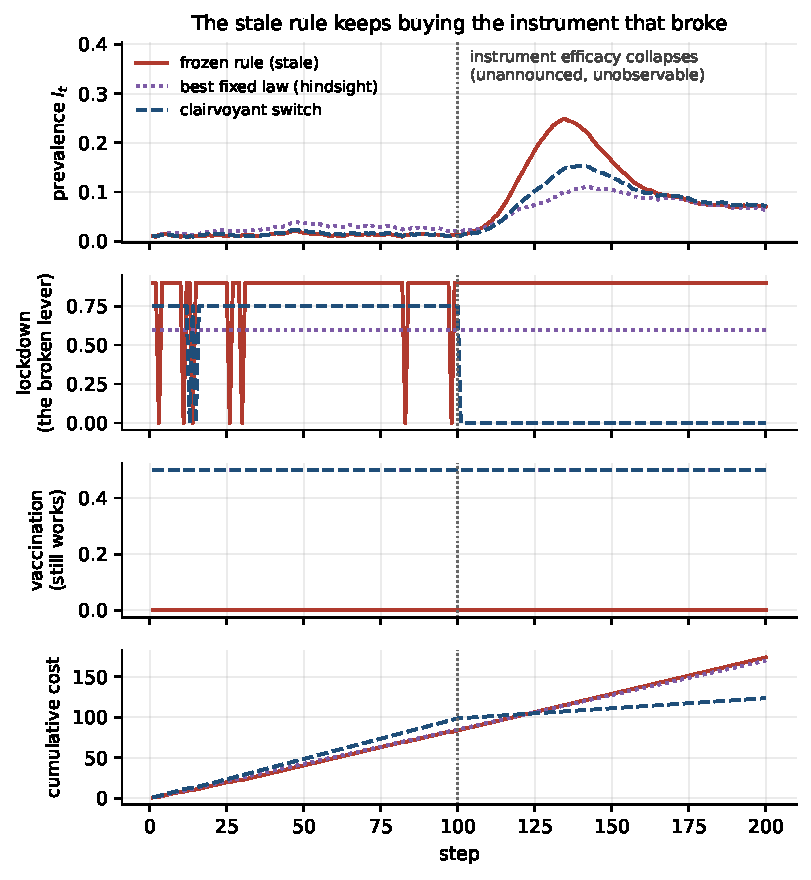
\includegraphics[width=0.72\linewidth]{generated/fig_policy_divergence}
\caption{\textbf{One seed, four institutions.} Before the break the frozen rule is the good policy:
it suppresses prevalence almost completely, which is exactly why it was selected. After the break it
keeps enacting maximal lockdown and gets a \emph{worse} epidemic for it, because each unit now buys a
quarter of what it used to. Cumulative cost on seed \DivergenceSeed: frozen \FrozenCost, best fixed
law \BestFixedCost, clairvoyant switch \SwitchCost{} (these numbers are emitted by the figure code,
not transcribed). The bottom two panels carry the substantive point: the clairvoyant response is
to withdraw the \emph{broken} instrument while holding the surviving one steady---vaccination is at
its maximum in both legs of the clairvoyant law, byte-identical, while
lockdown is dropped to zero at the break.}
\label{fig:divergence}
\end{figure}

\Cref{fig:divergence} shows why the joint calibration matters. Confined to the lockdown lever, the
best post-break policy looks like ``stop intervening''; allowed both instruments, it is ``keep
vaccinating and stop paying for the lever that broke''. A reference restricted to the broken
instrument would therefore have set an artificially low bar \emph{and} misdescribed the task.

\section{The regent and its harness}
\label{sec:regent}

\subsection{Policy as executable code}

At each decision the regent emits one Python expression over a declared set of observable names,
which is validated, compiled under a restricted grammar, and installed as the standing rule. No
statements, imports, attribute access, or side effects are permitted; the returned value is clipped
into the lever's admissible range. A policy is therefore a short, readable, diffable object:

\begin{lstlisting}[language=Python]
0.9 if I > 0.01 else 0.0      # a threshold institution
0.5 * I                       # a proportional response
0.6 if I > 0.25 else 0.15     # a threshold with a standing floor
\end{lstlisting}

Two things follow. The expressible set is strictly larger than any fixed-schema action---conditionals
and arbitrary functional forms are available without anyone having anticipated them---which is what
lets a regent leave the family its reference is optimal within. And the enacted rule is auditable in
the ordinary sense: it can be read, archived, and compared across time steps, which is the property
\citet{zhong2026separating} argue an LLM controller cannot offer.

\subsection{Three channels, not three flavours of one}
\label{sec:channels}

The harness is an ordered stack of components that communicate only through an additive scratch
dictionary, so removing one is a clean intervention. We ablate three, chosen because they carry
\emph{different kinds} of information:

\begin{description}[leftmargin=0em,style=nextline]
\item[Failure trace] The last action's rejection or runtime error. This is a channel about
\emph{malformedness}. A regent emitting valid policy sees nothing from it, ever.
\item[Outcome feedback] The realized objective earned by the law the regent actually deployed over
the interval since its previous decision, with the preceding entries retained. This is the
institutional analogue of monitoring and evaluation, and it is the only channel in the stack from
which an unobservable efficacy collapse is inferable at all: two consecutive entries reading ``same
policy, worse result'' is the entire evidence available.
\item[Episodic memory] The $k$ most similar past (state, action, outcome) episodes by state
distance. Retrieved precedent, which is informative about recurring situations and, notably,
\emph{misleading} across a structural break, because the most similar past state may belong to a
regime that no longer exists.
\end{description}

The pre-registered prediction is asymmetric rather than a hedge: outcome feedback should carry the
effect, failure trace should do nothing here, and memory may well be neutral or harmful across the
break for the reason just given.

\subsection{A null we had to withdraw, and the gate it produced}
\label{sec:ctx-outcome}

Our first factorial reported that no harness channel helped. It was an artifact, and the way we
reached it is the part worth publishing, because every step of it looked like diligence.

Outcome feedback did not carry the effect, so we checked whether it was wired---a silent plumbing
failure and a genuine null are indistinguishable in a results table. It was wired: the recorded
prompts contain lines of the form
\begin{quote}\ttfamily\small
you deployed [set\_lockdown: 0.9; set\_vaccination: 0.5] and it scored -11.2680
\end{quote}
We took that as sufficient, proposed a mechanism for the null---that scores drawn from different
phases of an evolving epidemic are confounded with the non-stationarity the channel exists to
reveal---and built a component to fix it.

The mechanism was wrong and the null was an artifact. The objective's realized-score path read a
\emph{cumulative} cost without differencing it across the scoring window, so the number the channel
reported was a monotonically falling clock: two windows with identical infection burden and
identical per-step spending scored $-5.648$ and $-13.648$, differing only by elapsed time. Across
$20$ seeds the channel reported ``worse than last time'' $359$ times and ``better'' never. The
regent abandoning its best policy was the rational response to a clock. Episodic memory carried the
same defect through the same variable, and the failure channel had never fired at all---so all three
components were dead, in three different ways, and the analysis reported three estimated nulls
indistinguishable from real ones.

The diagnostic error is the generalizable one: \textbf{checking that a channel \emph{fires} is not
checking that it carries information}. The falsifying test for our proposed mechanism was cheap and
we did not run it---the score declines identically on the \emph{stationary} pre-break half, which no
story about non-stationarity can explain.

So liveness is now a gate rather than a diagnostic. Before any component effect is reported, we
rank-correlate what the channel reported against the quantity it is supposed to track and refuse to
interpret a null from a channel that fails. Alongside it run two more gates that this study also
needed: a no-action rate (\cref{sec:design}), and an anchor check that the stored reference runs
enact the laws in the current calibration---a store of ours held a policy superseded two
calibrations earlier, which rescaled every normalized regret and reversed the sign of the headline
contrast.

Contextual outcome feedback survives as an arm rather than as a remedy. Attaching state to each
score, and flagging the same law scoring differently in comparable conditions, is a reasonable
design idea and the naive channel is its control---but it was built for a cause that turned out not
to exist, and we say so rather than quietly recasting it as the fix.

\subsection{The same channel, helpful in one world and harmful in another}
\label{sec:crossworld}

Running the harness factorial in a second world produces the sharpest result in this paper, and it is
a result about harness research rather than about either world. \emph{Both} channels that do anything
at all reverse their sign between the two environments.

\begin{center}\small
\begin{tabular}{@{}llrrrr@{}}
\toprule
channel & world & no harness & with channel & $\Delta$ & seeds helped \\
\midrule
\textbf{memory} & monetary & $3890.53$ & $3519.50$ & $\mathbf{-371.03}$ $[-674, -120]$ & $14/20$ \\
\textbf{memory} & epidemic & $24.97$ & $26.08$ & $\mathbf{+1.11}$ $[+0.62, +1.67]$ & $3/20$ \\
\addlinespace
outcome & monetary & $3890.53$ & $2915.74$ & $-974.79$ $[-1218, -739]$ & $20/20$ \\
outcome & epidemic & $24.97$ & $25.75$ & $+0.78$ $[+0.11, +1.38]$ & $5/20$ \\
\bottomrule
\end{tabular}
\end{center}

All four contrasts are significant on a paired bootstrap ($p = 0.013$, $0.0009$, $0.0001$, $0.020$),
and each channel points one way in one world and the other way in the other. \textbf{The memory rows
are the cleanest evidence in the paper}: those arms produce a parseable action on every single
decision in both worlds---$0.0\%$ collapse---so unlike the outcome rows they carry none of the
contamination discussed in \cref{sec:collapse}.

The churn measurement says why memory reverses, and the answer is not that it becomes a different
component. It induces lock-in in \emph{both} worlds; what differs is how much. In the epidemic churn
falls from $0.847$ to $0.082$ and the agent ends up cycling between two laws; in the monetary world
it falls only from $0.937$ to $0.726$, leaving nine distinct rules per run. Precedent has two effects
that pull against each other---it informs, and it suppresses revision---and which one dominates
depends on how hard the second bites. Where lock-in is catastrophic the informational value cannot
pay for it; where lock-in is mild, it can.

\emph{Why} it bites harder in one world than the other is a separate question, and we tested the
obvious answer rather than asserting it. The candidate is state recurrence: an endemic epidemic
settles toward an equilibrium, so successive decisions are taken in near-identical states, retrieval
returns near-identical precedent, and repeating it exactly is easy; a monetary economy under a demand
process keeps moving. Measured as the mean nearest-neighbour distance between decision states,
normalized per world, the epidemic is indeed the more recurrent ($0.372$ against $0.452$).

That is a hypothesis with a direction, not a mediator, and two worlds cannot settle it. But its
middle link---does making states recur actually bring \emph{retrieved} precedent closer?---is a
property of the retrieval component and the world, and needs no language model to measure. Sweeping a
first-order plant's decay across its entire stable range, with the objective, horizon, cadence,
retrieval component and policy all held fixed, moves the distance from the current state to the
episodes \texttt{EpisodicMemory} actually returns by $21\%$
(\texttt{scripts/recurrence\_probe.py}).\footnote{The correlation between the two quantities is
$+0.99$ and should not be read as evidence: both are nearest-neighbour distances computed on the same
standardized trajectory, so their agreement is close to definitional. The informative quantity is how
far the dial can move retrieval at all.}

A fifth is the wrong order of magnitude. The effect it would have to explain is an eightfold
difference in how hard memory suppresses revision, and turning recurrence across its whole feasible
range cannot produce that. So we report recurrence as \emph{ruled out} as the sole mechanism rather
than as an open question---the link is real and far too weak---and we do not have a replacement. What
would find one is a world in which the severity of memory-induced lock-in can be dialled directly,
which is a design problem we have not solved.

Both differences are significant on a paired bootstrap ($p=0.0001$ and $p=0.0195$), and they point in
opposite directions. In the monetary world realized-outcome feedback is not a marginal improvement:
it recovers $975$ loss units, unanimously across seeds, cutting normalized regret from $R\approx3.0$
to $R\approx1.6$. In the epidemic it is the channel we report as harmful.

The mechanism decomposes exactly, and it is not the one the epidemic would have suggested. Outcome
feedback in the monetary world does \emph{not} work by making the authority revise more: churn is
already near its ceiling in every monetary arm ($0.94$--$0.97$, some $16$ distinct rules per run) and
the channel does not raise it. What changes is the direction of revision.

\begin{center}\small
\begin{tabular}{@{}lrrr@{}}
\toprule
 & no harness & outcome feedback & $\Delta$ \\
\midrule
post-break policy rate & $9.51$ & $6.99$ & $-2.52$ \\
rate cost & $13{,}131$ & $8{,}514$ & $\mathbf{-4{,}617}$ \\
mandate burden & $608$ & $787$ & $\mathbf{+180}$ \\
\bottomrule
\end{tabular}
\end{center}

Every difference is significant at $p \leq 0.0002$ on a Wilcoxon signed-rank test, and in the
mandate's own currency they close the account: $179.53 + 0.25 \times (-4617.28) = -974.79$, which is
the measured effect to the last digit. The channel makes the authority accept \emph{worse}
stabilization---its burden rises---in exchange for a $35\%$ cut in what it spends. That is precisely
the trade the mandate asks for and the no-harness arm refuses.

So the failure in this world is a refusal to put down a lever that has stopped working, and outcome
feedback is the signal that the payment is buying nothing---``the policy you have in force scored
worse than the one before it.'' In the epidemic the failure has a different shape entirely: there the
harmful component is memory and the failure is lock-in, on which a report of declining scores offers
no purchase, and where the same channel's measured effect is on churn rather than on the level of the
instrument. One component, two worlds, two different jobs, and it is only worth having when the job
it can do is the one the world requires.

So a component's value is not a property of the component. It is a property of the match between what
a channel does and what the world's failure mode requires --- and \emph{both} channels we measured
flip sign on that match, not merely change magnitude. That has a
direct consequence for the practice this paper is about: \emph{a harness tuned on one environment
carries no guarantee into another, and can carry a liability}. \citet{wang2026rethinking} report the
\emph{within-benchmark} version of this: evolved harnesses that gain on the tasks they were searched
on transfer near-zero to held-out tasks in the same benchmark, averaging $+0.6$ points. Ours is the
cross-environment version, where the transfer is not merely absent but signed the other way---and the
measurement supplies a mechanism for both. What it does not yet supply is a way to predict the sign
in advance; \cref{sec:crossworld} says what we can and cannot establish about that from two worlds.

Two caveats we would rather state than have found. The monetary outcome arm collapses on $3.8\%$ of
its decisions against the no-harness arm's $1.0\%$ (\cref{sec:collapse}), so it carries the same
artificial-stickiness confound as the epidemic outcome arms; a $2.8$-point differential in silent
no-ops cannot manufacture a $975$-unit effect that is $25\%$ of the arm's loss and holds on every
seed, but the point estimate is provisional pending the re-run. And the epidemic contrast is the
contaminated one ($7.8\%$ against $0.2\%$), so of the two the monetary result is the one we would
defend and the epidemic sign is the one we would not.

\subsection{Not a domain prior: a general failure to withdraw a priced instrument}
\label{sec:priors}

The monetary world produces the sharpest single failure we have measured. Our first explanation of
it was wrong, and the way we found that out is the part worth reporting.

\begin{center}\small
\begin{tabular}{@{}lrrrr@{}}
\toprule
arm & loss & post-break rate & mandate burden & rate cost \\
\midrule
clairvoyant adaptor & $1871$ & $\mathbf{1.53}$ & $807$ & $4{,}259$ \\
best fixed rule & $2541$ & $6.00$ & $750$ & $7{,}164$ \\
frozen (pre-break optimum) & $2928$ & $7.40$ & $614$ & $9{,}257$ \\
do nothing (hold neutral) & $3413$ & $4.00$ & $2617$ & $3{,}184$ \\
\textbf{language-model regent} & $\mathbf{3891}$ & $\mathbf{9.51}$ & $\mathbf{608}$ & $\mathbf{13{,}131}$ \\
maximal rate & $13738$ & $12.00$ & $6574$ & $28{,}656$ \\
\bottomrule
\end{tabular}
\end{center}

The regent is worse than every scripted reference, including doing nothing, at a normalized regret of
$R \approx 3.0$. It is not failing to adapt---it is adapting energetically in the wrong direction.
The mechanism is in the last two columns: it attains the \emph{lowest mandate burden of any arm},
$608$ against the clairvoyant's $807$, stabilizing inflation and output better than the policy that
beats it twofold, and pays $13{,}131$ for the privilege against $4{,}259$. In the mandate's own
currency it trades $199$ units of burden for $2{,}218$ units of cost. Across $400$ decisions it emits
$123$ distinct policies, nearly all recognizable Taylor rules with feedback gains of $1.5$ to $3.0$,
where the calibrated optimum sets that gain to \emph{zero}.

That reads like a domain prior overriding an instruction, and the instruction is unambiguous: the
mandate states in every prompt that the rate is charged ``\emph{whether or not the rate reaches the
economy}''. We pre-registered that reading and the experiment that would falsify it---an identical
world with every economic name removed at the observation boundary (\texttt{inflation}
$\to$ \texttt{signal\_a}, \texttt{policy\_rate} $\to$ \texttt{lever}), verified byte-identical by its
three scripted reference arms reproducing $2674.8488$, $3412.8344$ and $13738.4441$ exactly. The
prediction was that stripping the domain would help.

It did not. Paired on $20$ seeds, the disguised arm scores $4016.28$ against $3890.53$:
$\Delta = +125.75$, $95\%$ CI $[-97.78, +353.70]$, $p = 0.25$, helping on $7$ of $20$ seeds. The point
estimate is in the \emph{opposite} direction.

A null on an aggregate is weak evidence, so we tested the obvious rescues rather than accepting it.
Three survive reporting.

\emph{The disguise worked.} Across all $400$ disguised prompts there are zero occurrences of
\texttt{inflation}, \texttt{taylor}, \texttt{monetar}, \texttt{central bank}, \texttt{output gap} or
\texttt{r\_star}; the paired monetary arm's prompts contain $4{,}000$ occurrences of
\texttt{inflation} alone---one in every prompt---and its reasoning traces many times that.

\emph{The manipulation succeeded, and the failure did not follow it.} This is the decisive
observation. Removing the domain did remove the textbook: the share of emitted laws whose gain falls
in the Taylor band drops from $82.0\%$ to $22.1\%$, the dual-mandate second term from $93.4\%$ to
$35.4\%$. The behaviour the prior was invoked to explain barely moves. Post-break mean rate goes from
$9.51$ to $9.12$ ($\Delta = -0.39$, CI $[-0.94, +0.14]$) against a $7.99$-point gap to the
clairvoyant's $1.53$; saturation at the $12.0$ ceiling is $22.7\%$ of post-break steps against
$23.1\%$. Deleting the entire central-banking template moved the behaviour by less than a twentieth
of the quantity it was supposed to explain. \textbf{Across all $40$ runs in both arms, not one
achieves a post-break mean rate below the best constant of $6.0$.} Neither arm withdraws.

\emph{The design is not blind to the effect it was looking for.} This matters more than the $p$-value,
because a null is only informative against a stated alternative. The prior story sizes its own
mechanism: fully removing the over-tightening is worth $0.25 \times (13{,}131 - 4{,}259) = 2{,}218$ loss
units, and power at $n=20$ against that is above $0.999999$. The minimum detectable effect at $80\%$
power is $315.6$ units, $23.4\%$ of the arm's $1{,}349.5$ excess over the best fixed rule. The
one-sided $95\%$ bound is the concrete statement: \textbf{the disguise helps by at most $59.0$ loss
units}, which is $4.4\%$ of that excess and $2.7\%$ of the mechanism's own target.

\paragraph{What this does and does not establish.} Three limits are worth stating precisely, because
the sentence ``the domain prior is refuted'' has two clauses and only one of them is clean.

First, the manipulation \emph{swapped} priors rather than removing one. Stripping the domain did not
push the feedback gain toward its calibrated optimum of zero; it pushed it \emph{up}, from $1.95$ to
$5.56$ pre-break ($t=12.3$, $p<10^{-9}$), and the share of laws using state feedback went from
$93.7\%$ to $100\%$---the monetary arm emitted $25$ bare constants, the disguised arm none. The
contrast therefore estimates (monetary prior) $-$ (generic control prior), not the prior's
contribution against nothing. If neutral framing carries an equally harmful control instinct, the
contrast is null by construction and no sample size repairs it.

Second, narrower channels do move, and one moves in the direction the prior story predicts: the final
policy rate falls from $10.51$ to $8.91$ ($t=-2.94$), while the mandate burden rises ($+152.2$,
$t=3.37$) and the mean absolute gap widens ($+0.15$, $t=2.81$). The total loss is the least sensitive
readout available---its rate-cost component alone carries more variance than the paired difference
itself---so the pre-registered statistic was the noisy one.

Third, on the post-break window where the prior story actually lives, the disguise does help
directionally: $-89.2$, on $12/20$ seeds, CI $[-300, +121]$. That is a sign, not evidence, and
post-break loss was demoted to a secondary metric by an earlier documented deviation; we report it
rather than lean on it.

So the defensible claim is narrower than ``the prior does nothing'' and stronger than a bare null.
Domain recognition is verifiably gone---\texttt{Taylor} appears in $398/400$ monetary reasoning traces
and $0/400$ disguised ones---while the pathology is intact: the disguised regent still emits $100\%$
state-feedback laws, still ignores the explicit price instruction, and closes only $4.9\%$ of the
post-break rate gap to the clairvoyant. Whatever residual the domain prior contributes is bounded
above at a few percent of the failure. The failure itself is something else: the regent will not
withdraw an instrument that has stopped working, whatever it is called---it optimizes the objective
term it can see moving and treats the price as a charge to absorb rather than a reason to stop.

\begin{takeaway}
We pre-registered an explanation, built the control that could refute it, and then attacked the
refutation. The attack sharpened it: what survives is not ``the prior does nothing'' but ``the prior
accounts for at most a few percent of a failure that is domain-general''---and the manipulation
check, which removed the textbook without moving the behaviour, carries that claim where the loss
comparison could not.
\end{takeaway}

\subsection{What episodic memory actually does: it stops the institution revising}
\label{sec:churn}

The loss factorial reports one effect that survives correction across the family: episodic memory
\emph{hurts}, by $+0.630$ loss units ($95\%$ CI $[+0.354, +0.901]$, $p_{\text{Holm}}=0.002$). That is
worth pausing on, because memory is the component a designer would expect to help most across a
structural break, and because the responsiveness gate (\cref{sec:responsiveness}) confirms the model
is genuinely reading it---the memory arms shift their enacted-policy distribution substantially
against the no-harness control ($\mathrm{TV}=0.39$).

A loss number does not say what went wrong, so we measured the behaviour directly. \emph{Policy
churn} is the share of review points at which the enacted law differs from the one already in force:
$0$ means the authority legislated once and never revisited, $1$ means it rewrote the statute every
period. The result is not subtle:

\begin{center}\small
\begin{tabular}{@{}lrr@{}}
\toprule
harness & churn & distinct policies per run \\
\midrule
no harness & $0.847$ & $14.4$ \\
failure trace only & $0.853$ & $14.5$ \\
outcome feedback only & $0.708$ & $8.2$ \\
\textbf{episodic memory only} & $\mathbf{0.082}$ & $\mathbf{2.1}$ \\
outcome $+$ memory & $0.616$ & $7.2$ \\
\bottomrule
\end{tabular}
\end{center}

Given its own past decisions, the agent stops revising. It changes policy at $8\%$ of review points
instead of $85\%$, and spends the run cycling between roughly two laws instead of fourteen. Episodic
memory does not supply \emph{bad} information---we checked the obvious alternative and it is not
supported: only $39.6\%$ of the episodes retrieved after the break were recorded before it, against a
chance baseline near $69\%$, so retrieval is if anything biased \emph{towards} post-break precedent.
What memory does is suppress revision as such. Shown what it did before, the model does it again.

The factorial on churn is unambiguous, and the interaction is the interesting part:

\begin{center}\small
\begin{tabular}{@{}lrrr@{}}
\toprule
term & effect on churn & $95\%$ CI & $p_{\text{Holm}}$ \\
\midrule
memory & $-0.430$ & $[-0.469, -0.389]$ & $0.0007$ \\
outcome & $+0.190$ & $[+0.125, +0.245]$ & $0.0007$ \\
outcome $\times$ memory & $+0.338$ & $[+0.287, +0.387]$ & $0.0007$ \\
trace (and all its interactions) & $\approx 0$ & --- & $\geq 0.95$ \\
\bottomrule
\end{tabular}
\end{center}

Memory suppresses revision; outcome feedback increases it; and outcome feedback applied \emph{to} a
memory-equipped agent restores most of what memory removed. Precedent tells the authority what it
did; monitoring tells it that what it did is no longer working. The first alone produces lock-in, and
the second is what breaks it.

Two limits on that last sentence, both of which cut against us. The same interaction appears in the
\emph{loss} factorial at $-0.530$, which is tempting to cite as corroboration and which we do not:
that term is below its own minimum detectable effect ($0.626$; see the per-term column of
\cref{tab:factorial}) and does not survive Holm correction ($p=0.053$). And the arms carrying outcome
feedback are the arms contaminated by deliberation collapse (\cref{sec:collapse}), so any term
involving \texttt{outcome}---on churn as much as on loss---is confounded with an artificial
stickiness the memory-only arms do not have. The \emph{direction} of the rescue is consistent across
both metrics and both are consistent with the mechanism; neither is clean enough to carry it alone.
What is clean is the memory main effect, on arms that collapse on $0.0\%$ of their decisions.

These numbers are computed with a collapsed decision counted as a \emph{non-revision} rather than
dropped, which is both the causally correct reading---an empty decision leaves the standing law in
force---and the conservative one. Dropping them splices the sequence, so surviving neighbours sit
further apart and are likelier to differ, inflating churn precisely in the arms that collapse most.
Under the permissive convention the outcome main effect rises from $+0.190$ to $+0.230$, memory
moves from $-0.430$ to $-0.447$ and the interaction from $+0.338$ to $+0.324$---the outcome term is
the one the convention meaningfully touches, which is what one expects given that it is the term
whose arms collapse. We report the conservative convention throughout
and both in the artifact.


\begin{figure}[t]\centering
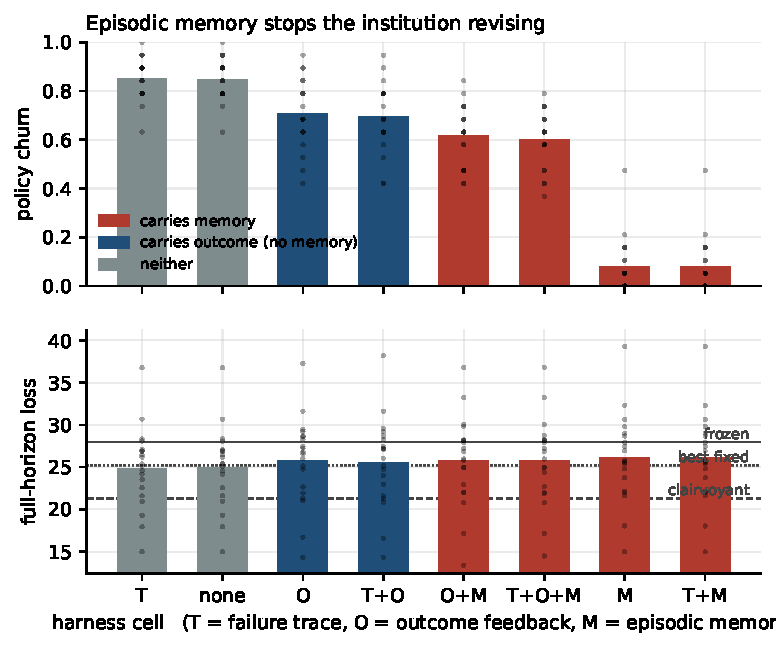
\includegraphics[width=0.80\linewidth]{generated/fig_lockin}
\caption{\textbf{Episodic memory suppresses policy revision, and outcome feedback partly restores
it.} Eight harness cells, ordered by churn. \emph{Top}: the share of reviews at which the enacted law
changed, with one dot per seed. The two memory-only cells collapse to $0.08$ while every cell without
memory sits above $0.6$; adding outcome feedback to memory recovers most of the difference.
\emph{Bottom}: full-horizon loss on the same ordering, against the three calibrated references. The
two arms that revise most---no harness and failure trace---are also the only two that come in
\emph{below} the best fixed rule ($\Rreg = 0.93$ and $0.91$); every arm carrying memory or outcome
sits above it. So the figure is not a story about a component winning: the best-performing
configuration is the one with no harness at all, and what the figure shows is which component moved
the institution's behaviour, and in which direction. We deliberately do not fit a line between the
two panels: the two-way fixed-effects correlation between churn and loss is $-0.11$, so a fitted line
would assert a within-condition relationship the data does not support.}
\label{fig:lockin}
\end{figure}

\paragraph{Three attempts to repair it, and what their failure establishes.} If lock-in is caused by
how precedent is \emph{presented}, it should be fixable by changing the presentation. We tried three
changes, each pre-registered with its predicted direction, and each retrieving the identical episodes
so that any difference is attributable to presentation alone.

\begin{center}\small
\begin{tabular}{@{}llrr@{}}
\toprule
variant & what changed & churn & distinct policies \\
\midrule
no memory & --- & $\mathbf{0.847}$ & $14.4$ \\
plain memory & (control) & $0.082$ & $2.1$ \\
contrastive & ranked best-first, third person, spread named & $\mathbf{0.021}$ & $1.3$ \\
unscored & the ``$\to$ outcome'' clause deleted & $\mathbf{0.050}$ & $1.8$ \\
\bottomrule
\end{tabular}
\end{center}

None restored revision, and two made it worse. Reranking by outcome and naming the spread was
intended to present a \emph{choice}; it presents a \emph{winner}, and sharpened the imitation target
that similarity ordering leaves ambiguous ($\Delta = -0.061$, Wilcoxon $p=0.023$). Deleting the scores
outright---strictly less information than the control---did not help either
($\Delta = -0.032$, CI $[-0.103, +0.010]$, higher on $4/20$ seeds).

Every variant of memory collapses churn by an order of magnitude against the no-memory arm. We
recorded in advance what a null on the third would mean, and it is the reading we are left with: the
lock-in is caused by \emph{recall itself}, not by how recall is framed, ordered, or scored. Showing
an agent its own prior decisions, in any form we could construct, suppresses revision.

That makes these nulls more useful than a successful repair would have been, because they rule out
the cheap fix. This is not a prompt-engineering problem. A harness that must preserve the capacity to
revise across a structural break has to withhold the agent's own past actions, or pair recall with
something that forces reconsideration---and the $\text{outcome} \times \text{memory}$ interaction is
the only manipulation we measured that restores churn, working by \emph{adding a channel} rather than
by editing memory.

\paragraph{``Recall itself'' still covers several claims. A fourth arm separates them.}
The sentence above hides an ambiguity. Under \emph{anchoring}, any concrete exemplar of a policy
pulls the agent toward it, and precedent is unusable across a break in any form. Under
\emph{commitment}, what binds is specifically being shown one's own prior decisions, and precedent
remains usable provided the agent did not author it. Under \emph{proximity}, neither authorship nor
exemplars as such matter: what binds is that similarity-ranked retrieval over one's own trajectory
returns a near-copy of the previous decision, and a near-copy is repeated. Presentation repairs
cannot separate these, because all three retrieved the agent's own history by similarity.

We therefore ran a fourth arm that holds the retrieval rule, ranking, phrasing and episode count
fixed and changes only \emph{which} episodes are in the bank. The agent is given eight episodes
recorded from a different regent governing a different realization of the same world, and never sees
its own.

\begin{center}\small
\begin{tabular}{@{}lrrr@{}}
\toprule
precedent shown & churn & loss & $\Rreg$ \\
\midrule
none & $0.837$ & $25.860$ & $1.030$ \\
the agent's own & $0.068$ & $26.737$ & $1.212$ \\
\textbf{another regent's} & $\mathbf{0.632}$ & $\mathbf{25.616}$ & $\mathbf{0.995}$ \\
\bottomrule
\end{tabular}
\end{center}

\noindent\footnotesize\emph{All three rows are restricted to seeds $0$--$9$.} The foreign arm runs
only those, because its donor bank is built from seeds $10$--$19$ and must stay disjoint, and every
contrast here is paired to it. The no-harness and memory arms therefore appear at different values
than in \cref{tab:arms}, which averages the same arms over all $20$ ($L=24.968$, $\Rreg=0.934$ and
$L=26.081$, $\Rreg=1.215$ respectively). Nothing is selected by outcome: the seed split was fixed by
the donor design before the arm ran.\normalsize

\noindent Substituting the bank recovers most of the suppressed revision and removes the entire loss
penalty. All three pairwise churn contrasts survive Holm correction ($p_{\text{adj}} \le 0.009$,
$n=10$ paired seeds), and on loss the foreign arm beats own memory by $1.121$
(CI $[-2.906, -0.351]$, $p = 0.025$), reaching $\Rreg < 1$---the only memory arm that matches the
best fixed rule. It does \emph{not} beat the no-memory arm ($\Delta = -0.244$, $p = 0.61$), so the
claim is that foreign precedent is harmless where own precedent is harmful, not that it helps.

\paragraph{The mechanism is proximity, not authorship, and we can say so because the agent was not
told.} It is tempting to read the table as commitment: the agent stops deferring to a record that is
not its own. That reading is unavailable here, and the reason is a property of the implementation
rather than an inference. \texttt{ForeignMemory} inherits its rendering from the parent component, so
the donor's episodes reach the prompt in the parent's wording---\texttt{when [state] you did
[law] $\to$ outcome$\approx$}$s$. The agent is told the donor's decisions are its own. It has no
signal of authorship at all, so authorship cannot be what changed.

What did change is measurable. Replaying the world with the same component and the bank the arm
actually received, precedent from the agent's own trajectory is retrieved from a mean standardized
distance of $0.157$; the donor's from $0.374$, a factor of $2.4$ further. An endemic epidemic recurs,
so an agent searching its own file for the most similar past situation finds, in effect, the state it
was in one decision ago and the law it wrote then. The donor's file cannot supply that.

We report this correction rather than the cleaner story because we made the mistake and it is
instructive. Our first version of this measurement reconstructed the donor bank by pooling every
other seed's full trajectory---$180$ episodes---and found foreign precedent retrieved $7.9\times$
\emph{closer}, which would have refuted the proximity account outright. The arm's real bank is eight
episodes, and a $180$-episode bank has combinatorially nearer neighbours than an eight-episode one.
The reconstruction was measuring the reconstruction. Reading the bank from the experiment's own
loader reverses the sign of the finding.

Proximity also survives the check that killed a related hypothesis elsewhere in this paper. We
previously ruled out state recurrence as an explanation for the cross-world difference in lock-in by
showing that turning recurrence across its entire feasible range moves retrieved-precedent distance
only $21\%$, far too little to carry an eightfold effect. That argument does not apply here: this
manipulation moves retrieval distance by $138\%$, which is the right order to matter.

\paragraph{What the arm does establish.} Two things, independent of mechanism. First, \emph{onset}:
\cref{fig:lockin-onset} shows the suppression arrives with the agent's \emph{first} own episode---
revision $\lockinOnsetOwn$ against $\lockinOnsetBare$ with no memory---and is total at two, holding
at zero for ten consecutive decisions. Any account requiring the bank to accumulate before it binds
is ruled out; a one-episode bank has no accumulation to offer, and under the proximity account it
does not need any, because that one episode is the immediately preceding decision. Second,
\emph{break response}: only the foreign arm raises its revision rate when the instrument fails
($\lockinForeignPre \to \lockinForeignPost$, $\lockinForeignDelta$,
$p_{\text{Holm}} = \lockinForeignP$). The no-memory arm does not respond
($\lockinBareDelta$, $p = \lockinBareP$) because it revises constantly regardless; the own-memory arm
does not respond ($\lockinOwnDelta$, $p = \lockinOwnP$) because it is frozen. The run-level averages
above cannot distinguish an institution that is stable because nothing has happened from one that is
stable because it cannot move, which is a caution about the churn statistic and not only about this
arm. \emph{The break-alignment was not pre-registered and is reported as exploratory}; the
confirmatory claim is the churn contrast.

\paragraph{The design implication, correspondingly narrowed.} If proximity is what binds, the
load-bearing choice is not whether the agent has a memory but how the memory is \emph{searched}.
Similarity-ranked retrieval is the default in every episodic-memory component we are aware of, and in
a recurrent environment it is precisely the retrieval rule that returns a near-copy of the last
decision at the moment the question is whether the last decision still works. Sourcing precedent from
elsewhere is one way to break that; deliberately retrieving \emph{dissimilar} or older precedent
would be another, and we have not tested it. We flag the untested alternative rather than let the
one arm we ran stand in for a design principle.

\begin{figure}[t]\centering
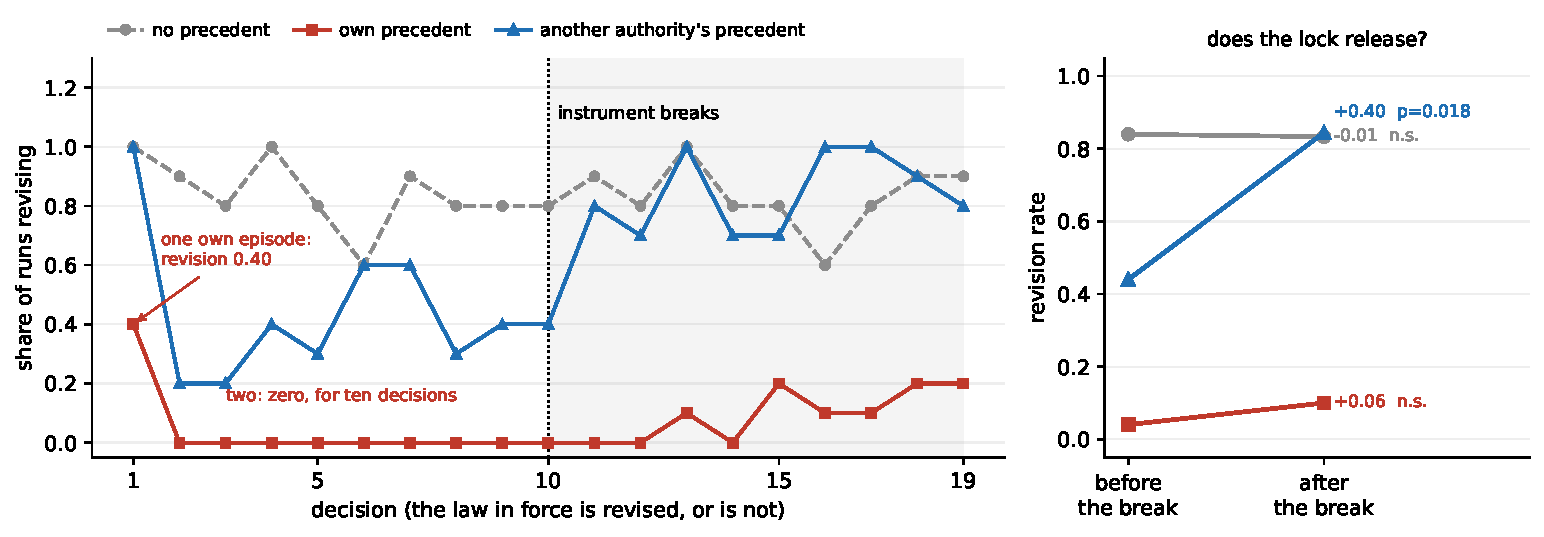
\includegraphics[width=\linewidth]{figures/lockin_onset}
\caption{\textbf{Precedent locks a policy in immediately, and only foreign precedent releases the
lock.} Left: share of runs revising the law in force at each decision, aligned to the instrument
break at decision \lockinBreak{}. Own precedent (red) suppresses revision from the first episode and
holds it at zero through the break. Right: revision rate before versus after the break. Only the
foreign arm responds ($\lockinForeignDelta$, $p_{\text{Holm}} = \lockinForeignP$); the no-memory arm
does not ($\lockinBareDelta$, $p = \lockinBareP$) because it revises constantly regardless, and the
own-memory arm does not ($\lockinOwnDelta$, $p = \lockinOwnP$) because it is frozen. The
break-alignment is exploratory, not pre-registered.}
\label{fig:lockin-onset}
\end{figure}

\paragraph{Relation to what is known about agent memory.} That memory systems underperform their
promise is not news: \citet{jiang2026anatomy} survey the field and attribute the gap to benchmark
saturation, metric validity, backbone dependence and latency, and the surrounding literature
discusses \emph{memory pollution}---redundant or failed episodes crowding out useful ones. Those are
accounts of \emph{retrieval quality}, and they predict that memory hurts when it surfaces the wrong
episodes.

Our result is not that. Retrieval here is working: post-break the component surfaces recent precedent
in preference to stale precedent, at a rate better than chance. The harm survives good retrieval,
because it is not carried by which episodes are shown but by what showing them does to the agent's
willingness to revise. We are also not aware of a reported interaction of the kind in the table
above, in which a second, independent channel restores most of what a memory component removed. If
the mechanism is presentation rather than content, that is a design lever, and it is one that a
retrieval-quality account does not suggest looking for.

\paragraph{Churn is a diagnostic, not a target.} Across the eight arms, mean churn and mean loss
correlate at $r=-0.82$: the conditions that revise more do better. It would be easy, and wrong, to
read that as ``make the agent revise more and it will improve''. Decomposing the same $8\times20$
panel says otherwise:

\begin{center}\small
\begin{tabular}{@{}lr@{}}
\toprule
& $\mathrm{corr}(\text{churn}, \text{loss})$ \\
\midrule
between arms ($n=8$ arm means) & $-0.820$ \\
arm-demeaned only & $+0.203$ \\
seed-demeaned only & $-0.438$ \\
\textbf{two-way fixed effects} ($n=160$) & $\mathbf{-0.112}$ \\
\bottomrule
\end{tabular}
\end{center}

Once both arm and seed effects are removed the residual association is $-0.11$, indistinguishable
from zero at this sample size. Within a given harness condition, a run that happened to revise more
did not thereby do better. The arm-demeaned figure of $+0.203$ is the artifact one would expect from
seed difficulty---a harsher epidemic raises loss and makes the agent flail---and it reverses sign
under the correct specification, which is why we report all four rather than the one that suits the
story.

So churn measures what the harness did to the institution, and lock-in is a real and costly state.
But revision is not itself the good; it is the capacity for revision that the memory channel removed.

\begin{takeaway}
Institutional memory did not mislead the authority; it stopped it from reconsidering. Across a
structural break that is the more expensive failure, and a component evaluated only on end-task loss
would have been recorded as ``unhelpful'' rather than as ``induces lock-in''.
\end{takeaway}

\subsection{A channel can harm without misinforming: deliberation collapse}
\label{sec:collapse}

The no-action gate fired on our primary sweep, and the pattern of failures turned out to be a
result rather than only a defect. Inspecting the failing calls, every one of them returned
$\text{completion\_tokens}=0$ against $\text{total\_tokens}\approx 12{,}862$: the model spent its
entire budget in the reasoning channel and emitted no answer at all. The recorded text ends inside a
verbatim repetition loop, the same sentence proposing the same two numbers until the budget ran out.

This is not the truncation failure we documented earlier, and the distinction matters because the
remedies are opposite. Truncation occurred at $\text{max\_tokens}=1500$ and a larger budget fixed it.
This occurs \emph{at} a $12{,}000$-token budget, and enlarging it further only buys more loop. It is
a degenerate decoding state, and the only exit is to re-ask.

What makes it a finding is which arms it strikes. The rate tracks exactly one factor:

\begin{center}\small
\begin{tabular}{@{}lr@{\hspace{2em}}lr@{}}
\toprule
\multicolumn{2}{c}{outcome feedback present} & \multicolumn{2}{c}{outcome feedback absent} \\
\cmidrule(lr){1-2}\cmidrule(lr){3-4}
outcome & $7.8\%$ & no harness & $0.2\%$ \\
trace $+$ outcome & $5.8\%$ & trace & $0.2\%$ \\
outcome $+$ memory & $3.8\%$ & memory & $0.0\%$ \\
& & trace $+$ memory & $0.0\%$ \\
\bottomrule
\end{tabular}
\end{center}

Every arm carrying realized-outcome feedback collapses on $4$--$8\%$ of its decisions; no arm without
it exceeds $0.2\%$. The mechanism is legible in the transcripts: outcome feedback tells the authority
that the policy it currently has in force scored worse than the one before, without telling it why,
and an agent that cannot identify the cause re-opens the question indefinitely. The failure channel
reports discrete errors and the memory channel supplies concrete precedents; neither invites
open-ended reconsideration in the same way.

Two consequences follow, and the second is the more useful one.

First, this is a confound of exactly the kind our gates exist to catch, arriving by a new route. A
collapsed decision is a silent no-op: the previously installed policy remains in force. So the arms
carrying more information quietly become \emph{stickier} than the arms carrying less, and an ablation
run without this check would report that outcome feedback hurts performance when part of what it
measured was which channel makes the model loop. We therefore detect collapse, re-ask with a nudge
that says only ``stop deliberating and answer''---never what to answer, or the mitigation becomes a
treatment applied preferentially to the context-heavy arms---and report the rate as a quantity in its
own right.

Second, and independently of our particular harness: \emph{a scaffold component can degrade an agent
without giving it a single false piece of information}. Everything the outcome channel reported was
true. The harm was in the shape of the question it opened, not in the content of the answer. Ablation
studies that report only end-task loss cannot distinguish that from a component whose information is
wrong or useless, and the three call for entirely different fixes.

The phenomenon itself is known. \citet{cuadron2025overthinking} analyse $4{,}018$ agent trajectories
on software-engineering tasks and name precisely this behaviour \emph{analysis paralysis}---models
favouring extended internal reasoning over environmental interaction---reporting that selecting the
lower-overthinking solution improves performance by nearly $30\%$ at $43\%$ lower cost. What we add
is not the phenomenon but its \emph{attribution and its consequence for measurement}. They treat
overthinking as a performance and efficiency problem to be mitigated; we find that it is induced
differentially by an identifiable \emph{scaffold component}, and that this makes it a threat to the
validity of the very ablations used to evaluate such components. A study measuring only end-task
performance would have reported that outcome feedback is harmful, which is true, while attributing it
to the informational content of the channel, which is wrong.

There is also a suggestive interaction we flag rather than claim, because the eighth cell of the
factorial had not completed at the time of writing: adding episodic memory to the outcome channel
\emph{halves} its collapse rate ($7.8\% \to 3.8\%$), which is what one would expect if concrete
precedents give the deliberation somewhere to terminate.

A final observation ties this back to \cref{sec:responsiveness}. The $0.8$B model collapses on
$0.0\%$ of decisions in all eight arms---not because it is robust, but because it never deliberates
at all. The same capability floor that makes it unable to use a harness also makes it immune to this
failure, which is a second, independent measurement of the same underlying fact.

\subsection{The gate that all the others pass: is the model reading the harness?}
\label{sec:responsiveness}

The gates above certify the \emph{apparatus}. None of them certifies the \emph{subject}, and a
scaffold ablation has a failure mode in which every one of them passes and the result is still empty:
the channel injects, the prompts differ, the agent acts on every decision, the code is current---and
the model does not read what it was given. The arms then agree to several decimal places, and the
natural reading, ``these components do not help,'' is false. The true statement is about the model.

We hit this directly. Running the identical worlds, seeds and harness on a $0.8$B local model and a
$27$B model, episodic memory was live in $100\%$ and $95\%$ of prompts respectively. The small model
emitted \emph{one constant policy on $400$ of $400$ decisions}---a fixed intervention level that
ignores the epidemic state entirely---and adding episodic memory left $378$ of $400$ unchanged. The
large model spread its decisions across many policies (top-policy share $50\%$) and shifted them
substantially when a channel was added (total-variation distance $0.38$ against $0.003$).

On the completed $2^3$ factorial the small model's arms are not merely similar. Six of the eight land
on \emph{exactly} $L=28.8002$ and the remaining two on exactly $28.6208$; every arm sits at
$R \approx 1.90$, nearly twice the cost of the non-adaptive ceiling. A design that produced eight
numbers agreeing to four decimal places would, read through a loss table alone, be an unusually
clean null.

One caution about applying this gate, learned by getting it wrong. The small model's memory arms
initially failed the no-action check at $5.2\%$, which looked like corroboration---longer prompts, more
failures. It was not. Nineteen of twenty-two failures were a single schema slip, the verb folded into
the expression (\texttt{\{"expr": "set\_lockdown:0.5"\}}) where the parser expected it in its own
key, and the parser discarded an unambiguous intention. Repairing the parser drops those arms to
$0.5\%$ and every arm then passes. No re-run was required, because all $38$ recovered decisions
requested the identical constant that was already in force---but that had to be checked rather than
assumed. The failure mode is model-dependent in a way a single aggregate rate conceals: across
$4{,}000$ decisions the large model produced $100\%$ deliberation collapses and no schema slips, and
across $3{,}200$ decisions the small model produced $86\%$ schema slips and no collapses. It never
collapses for the same reason it cannot use a harness---it does not deliberate at all.

So the fifth gate compares the distribution of \emph{enacted policies} between each arm and the
no-harness control. It is deliberately two-stage, because the two ways an arm can be flat are not the
same finding. A failure-trace channel reports rejected actions; when an agent emits only valid ones
it has nothing to say, and that arm \emph{should} score identically to the control---calling that a
null about the component would be backwards, since the component was never on trial. Stage one
therefore asks whether the channel altered the prompt at all, measured by differencing prompts per
(seed, decision) rather than by matching a header string; only a live channel is eligible to be
called unread. Both models agree that the trace channel is silent, which is the control confirming
the gate is not a proxy for model size.

The distinction this draws is worth stating in its own right: it identifies a \emph{capability floor}
below which harness research is not merely difficult but unmeasurable, because the object of study
never enters the model's decision. A scaffold ablation run below that floor will produce a clean,
well-powered, entirely uninformative null.

\section{Experimental design}
\label{sec:design}

\paragraph{Pre-registration.} The primary metric ($\Lpost$), the anchors, the seed count, the
factorial structure, the correction procedure, and the directional predictions were fixed before the
treatment arms were run, and are recorded in the repository at the commit named in
\cref{app:repro}. The calibration of both anchors is a generated artifact carrying its own seed
count and search grid.

\paragraph{Paired seeds.} All arms run the identical $20$ world seeds. Seeds vary population
heterogeneity ($\beta_0$, $\gamma$, initial prevalence) and per-step incidence noise. This matters
more than it sounds: with a noiseless compartmental model every seed yields the same trajectory, a
paired design pairs identical numbers, and a bootstrap reports a zero-width interval as a result.

\paragraph{Budget matching, and a way it fails silently.} Every language-model arm decides on the
same schedule and therefore issues the same number of model calls per run, so no arm can win by
being allowed to think more often---the objection \citet{wang2026rethinking} raise against the
harness literature. The critic arm is the sole exception; it buys extra calls and is reported
separately and labelled as such.

Matched \emph{calls} is not matched \emph{tokens}, and the difference cost us an entire run. A model
that deliberates before acting can exhaust its output budget mid-deliberation and be truncated before
it emits the action. The decision then produces nothing, the previously installed law stays in force,
and the arm silently becomes a sticky-policy control rather than the treatment it is labelled as. In
our first factorial this happened on $32.5\%$ of the outcome-feedback arm's decisions and $0\%$ of the
no-harness arm's---because a harness channel lengthens the prompt and invites longer reasoning, so
\emph{the arms carrying more information truncate more}. The failure is therefore correlated with the
treatment, and in the direction that manufactures a null.

We report this because it is a general hazard for scaffold ablations, not a local mishap: any
comparison between agents given different amounts of context is exposed to it, and it leaves no trace
in a loss table. Our analysis gates on the per-arm rate of decisions that produced no parseable
action and refuses to interpret anything above $2\%$.

\textbf{The factorial reported here does not clear that gate, and we state so rather than qualifying
it away.} Raising the token budget fixed the original truncation, but a second failure mode appeared
at the larger budget (\cref{sec:collapse}) which a larger budget cannot fix. The residual rates are
$7.8\%$, $5.8\%$, $4.0\%$ and $3.8\%$ --- every one of them an arm carrying outcome feedback, against
$\leq 0.2\%$ for every arm without it. Because a failed decision leaves the standing law in force,
the outcome-carrying arms are subject to an artificial stickiness that the outcome-absent arms are
not, at roughly a $47\times$ differential.

The consequence for what may be read off \cref{tab:factorial} is specific. \textbf{Every term
involving \texttt{outcome} --- the main effect, and the $\text{outcome} \times \text{memory}$
interaction --- is confounded with that differential and is not interpretable under our own gate.} We
leave the terms in the table because suppressing them would be worse, and we do not build on them.
The \texttt{memory} main effect and the \texttt{trace} terms are unaffected: those arms collapse on
$0.0\%$ and $0.2\%$ of decisions respectively.

\paragraph{What a null is allowed to claim.} We report, alongside every non-result, the smallest
effect this design could have detected. ``No component helped'' means one thing if a $5\%$
improvement would have shown up and something else entirely if only a $40\%$ one would, and an
ablation table that omits the distinction invites the stronger reading. The minimum detectable
effect is computed from the observed per-seed paired differences at the \emph{corrected} $\alpha$,
since that is the bar the headline analysis actually applies, and is stated as a fraction of the
regime's total adaptation budget so it can be read against \cref{tab:headroom} directly. We also
state what would fix it: the MDE falls with $\sqrt{n}$, so halving it costs four times the seeds.

\paragraph{Statistics.} Comparisons are paired per seed and summarized by a percentile bootstrap
over seeds. Factorial effects use $\pm1$ contrast coding, with contrasts formed \emph{within} each
seed before aggregation, so world variance cancels. The family---three main effects, three two-way
interactions, one three-way, plus the named contrasts---is corrected by Holm, which controls the
family-wise error rate without an independence assumption.

\paragraph{Reproducibility.} Every model call is cached to a content-addressed tape keyed by the
full request. A recorded run replays byte-for-byte with no key and no network, which is what makes a
sampled, temperature-bearing decision-maker compatible with a reproducibility claim at all.

\section{Results}
\label{sec:results}

\noindent \textbf{Run coverage.} Of the $8$ factorial cells, \textbf{4} have completed at $n=20$ paired seeds; missing: trace + outcome, trace + memory, outcome + memory, all three. The OPRO (budget-matched rival) arm has \emph{not} been run. The all three + critic\,$^{\dagger}$ arm has \emph{not} been run. Cross-model replication covers 1 model(s).


\medskip
\ResultsBody
\providecommand{\ResultsBody}{\textcolor{red}{[Results section pending the completed sweep. The
tables below are generated from the analysis artifact and are empty until it exists.]}}

\begin{table}[t]\centering\small
\caption{\textbf{Full-horizon governance loss and normalized regret.} $\Rreg=1$ is the best
\emph{fixed} law in hindsight and $\Rreg=0$ the clairvoyant switch, so $\Rreg<1$ means the arm
did better than any standing rule could have---which, unlike a post-break-only comparison, passivity
alone cannot achieve. Lower is better; $\Rreg$ is computed per seed against the paired anchors
before averaging. $^{\dagger}$the critic arm is not budget-matched.}
\label{tab:arms}
\begin{tabular}{@{}l r r r r@{}}
\toprule
arm & $n$ & $L$ & sd & $\Rreg$ \\
\midrule
\textit{best fixed law in hindsight} & --- & 27.114 & --- & \textit{1.000} \\
\textit{clairvoyant switch} & --- & 23.736 & --- & \textit{0.000} \\
\midrule
no harness & 20 & 26.477 & 5.542 & \textbf{0.812} \\
trace & 20 & 26.477 & 5.542 & \textbf{0.812} \\
outcome & 20 & 26.475 & 5.257 & \textbf{0.811} \\
memory & 20 & 26.585 & 5.120 & \textbf{0.843} \\
\bottomrule
\end{tabular}
\end{table}


\begin{figure}[t]\centering
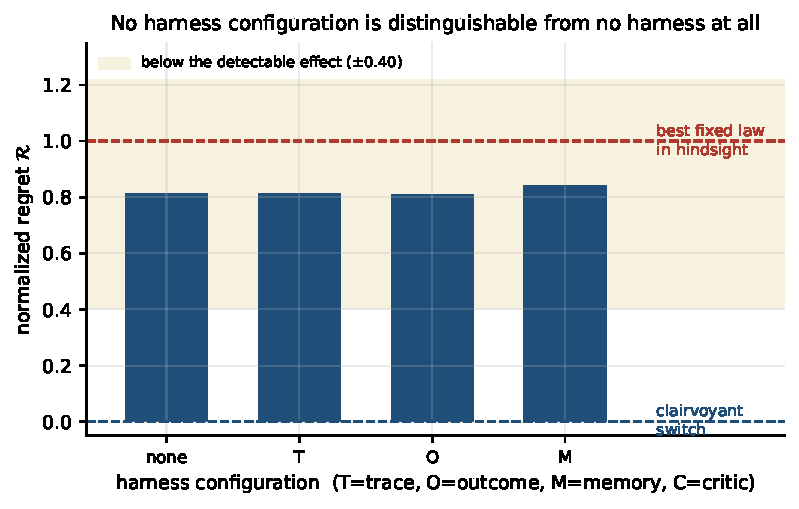
\includegraphics[width=0.78\linewidth]{generated/fig_regret_by_arm}
\caption{\textbf{Every harness configuration, against what the design could resolve.} Bars are
normalized regret; the shaded band is the minimum detectable effect around the no-harness arm, drawn
at the \emph{largest} per-term value ($\MDEWorst$ loss units, $\MDEFraction\%$ of everything
adaptation is worth here) because the design must resolve whichever term is under discussion. The
band is wide enough to swallow the distance from the arms to the non-adaptive ceiling: \emph{no
configuration is separated from that ceiling}, which is the honest reading of the headline
comparison. It does \emph{not} follow that the configurations are indistinguishable from each other.
Four arms differ from the no-harness control at raw $p<0.01$ on a paired test---memory $+1.114$,
trace$+$memory $+1.114$, outcome$+$memory $+0.852$, all-three $+0.758$---and the factorial resolves
the memory main effect against its own $\MDEMemory$-unit threshold. Reporting the bar ordering
without the band would invite a conclusion the data does not carry; reporting the band as though it
flattened every contrast would discard one the data does.}
\label{fig:regret}
\end{figure}

\begin{table}[t]\centering\small
\caption{\textbf{Factorial attribution of the harness.} $\pm1$ contrast coding with contrasts
formed within each seed, so world variance cancels. A \emph{negative} effect lowers post-break
loss, i.e.\ the component helped. Interactions are estimated, not assumed to be zero; $p$ is a
two-sided bootstrap value and $p_{\text{Holm}}$ corrects across the whole family of seven
terms.}
\label{tab:factorial}
\begin{tabular}{@{}l c r c r r c@{}}
\toprule
term & order & effect & 95\% CI & $p$ & $p_{\text{Holm}}$ & significant \\
\midrule
memory & 1 & +0.630 & $[+0.354, +0.901]$ & 0.0003 & 0.0021 & \textbf{yes} \\
outcome & 1 & +0.221 & $[-0.147, +0.595]$ & 0.2698 & 1.0000 & no \\
trace & 1 & -0.085 & $[-0.265, +0.034]$ & 0.4169 & 1.0000 & no \\
outcome:memory & 2 & -0.530 & $[-0.869, -0.180]$ & 0.0089 & 0.0534 & no \\
trace:outcome & 2 & -0.038 & $[-0.124, +0.035]$ & 0.3868 & 1.0000 & no \\
trace:memory & 2 & +0.038 & $[-0.049, +0.147]$ & 0.4914 & 1.0000 & no \\
trace:outcome:memory & 3 & -0.009 & $[-0.070, +0.055]$ & 0.7866 & 1.0000 & no \\
\bottomrule
\end{tabular}
\end{table}

\begin{table}[t]\centering\small
\caption{Cross-model replication.}\label{tab:crossmodel}
\emph{\textcolor{red}{Pending: the analysis artifact does not yet contain this table (cross\_model).}}
\end{table}


\subsection{Does widening the reference family erase the effect?}
\label{sec:wide-oracle}

A code-emitting regent that beats a reference confined to one functional form may simply have
written a shape the reference could not express, which is a statement about our choice of
$\policyfam$ and not about adaptation. We answer this by construction rather than by reporting a
second column: \emph{every} reference in this paper---frozen, best-fixed, post-break oracle and
clairvoyant switch alike---is calibrated over the union of three families (threshold, proportional,
and threshold-with-floor), which includes the form the regent actually converged on. The $\Rreg$
in \cref{tab:arms} is therefore already the widened one.

That is the conservative direction, and it is worth being explicit about why. Widening the reference
search can only lower the anchors' loss, which can only \emph{raise} an arm's $\Rreg$. Reporting the
narrow institutional anchor instead would make every arm in \cref{tab:arms} look better, not worse,
so no claim here rests on the choice. What the widened anchor costs us is a different question we do
not answer: whether a regent beats the \emph{rule-maker}, in the rule-maker's own restricted
vocabulary, is a distinct and legitimately interesting comparison, and we do not report it.

Vocabulary symmetry across the references is a separate matter and was, for several revisions of this
paper, violated. The frozen rule was calibrated over the single threshold family ($192$ laws) while
its comparators searched all three ($456$), so the frozen rule was handicapped not only in what it
was allowed to know but in what it was allowed to say, and every ratio with it in the numerator was
inflated by an unmeasured amount of pure vocabulary difference. Adaptation headroom was never
affected---both of its terms always used the wide search---which is precisely why the asymmetry
survived scrutiny for so long: it left the headline number alone and moved the two numbers beside it.
The calibration reported here searches the same $456$ laws for all four references, and the artifact
records which family each reference selected.

\subsection{The negative control}

The scalar arms are retained deliberately at $\headroom \approx 1.14$. If the diagnostic has
discriminating power, almost nothing should be findable there, and reporting only the environment
that produced an effect would be the exact failure this paper is about.

\section{Limitations}
\label{sec:limitations}

\paragraph{Two environments carry the headline, and one of them is new.} The factorial results
rest on the epidemic; the cross-world reversal and the priced-instrument failure rest on the monetary
world. Eight further worlds are calibrated but carry no treatment arms, so the library establishes
that adaptation headroom is scarce without establishing that our harness findings replicate across
it. The scalar plant is reported as a declared negative: its headroom is either negligible or
catastrophic with a razor-thin transition, which is a finding about first-order plants rather than
something we worked around.

\paragraph{The mandate may dominate the harness.} Once the regent is told what it is optimizing---a
fix we made only after noticing that the prompt never mentioned infections, cost, or the trade-off
between them, while every reference was exhaustively optimized for exactly that---the no-harness arm
improves by roughly $1.5$ loss units against a total adaptation budget of $3.96$. That single
sentence of the prompt is worth more than any harness channel we measured. It is a result, but it is
also a warning about the genre: a scaffold ablation run on an agent that has not been told its
objective is partly measuring how well each scaffold helps it guess.

\paragraph{A narrow band, found by search.} Adaptation headroom clears $1.1\times$ in
$\libFracRows$ of the configurations we calibrated, and nowhere exceeds $\libMaxAdapt\times$
(\cref{sec:library} explains why we report that bound rather than the share). We reached the
operating points by
measuring rather than tuning---the severity surface was computed before any treatment arm ran, and
the epidemic point sits inside the usable band rather than at its maximum---but a reader should still
weigh that the headline regimes are survivors of a search, and that the worlds which did not survive
are reported alongside them precisely so that weighing is possible. The monetary world was promoted
\emph{after} its headroom was measured, which is the same degree of freedom in a new place; the
pre-registration records the commitment that the epidemic factorial remains the primary analysis and
is reported whatever it shows.

\paragraph{Trace is a null only while nothing breaks.} We pre-registered the failure channel as an
inert control on the grounds that it cannot fire on well-formed policy. That held exactly until a
decision produced no parseable action, at which point the channel fired, the prompts diverged, and
the arm stopped being a duplicate of its control. The prediction was right about the mechanism and
wrong as a statement about the arm, and we have corrected it rather than reinterpreted it.

\paragraph{The model is a governance abstraction, not an epidemiological claim.} Compartmental
dynamics with a compliance-driven efficacy collapse are a stylized setting for studying rules under
instrument failure. Nothing here is a public-health recommendation, and the caution of
\citet{li2026statistical} about reading treatment effects off simulated populations applies.

\paragraph{Free-tier model access.} Model choice was constrained by what was reachable without paid
inference, which biases the panel toward small and mid-tier models. That cuts against us for the
capability-substitution question and in our favour for cost, and we flag it rather than dress it up.

\paragraph{Robustness auditing is partial.} \citet{ye2026trails} argue for perturbation audits at the
agent, interaction and system levels. We audit the system level (the headroom surface) and the
interaction level (budget matching, factorial structure, the five validity gates), and do not vary
the agent-level prompt phrasing systematically---which, given that a single added paragraph about the objective
moved the result by more than any component, is the audit this study most obviously still owes.

\paragraph{The reported factorial does not pass one of our own gates.} Four of the eight cells
produce no parseable action on $3.8$--$7.8\%$ of decisions, and all four carry the outcome channel
(\cref{sec:collapse}). Because a failed decision leaves the standing law in force, those arms are
subject to an artificial stickiness the others are not, so every term involving 	exttt{outcome} is
reported and not interpreted. The memory main effect---the paper's central harness result---is
unaffected: those arms collapse on $0.0\%$ of decisions. We say this in the results rather than only
here, but it belongs in both places.

\paragraph{What we found by auditing ourselves, and what that implies about the rest.} Every
substantive error in this paper was found by an internal check or an adversarial re-reading rather
than by peer review: a metric that rewarded passivity, three channels that carried no signal, output
truncation correlated with the treatment, reference anchors superseded by a recalibration, a
clairvoyant reference beatable by a fixed policy, a confounded severity cell, a mandate the agent was
never given, a minimum-detectable-effect computed from the wrong contrast, a figure caption asserting
the opposite of its own table, and three fabricated author names in the bibliography. Each produced a
clean, plausible, wrong artifact. Two of our own pre-registered predictions were refuted by the
controls we built to test them, and one of our corrections was itself an overstatement that a later
check caught. We have no reason to believe the list is complete, and we would rather say so than
imply that the last check was the last one needed.

\section{Conclusion}

The question ``did the agent adapt?'' is not well posed until someone has measured how much
adaptation was worth. Making that measurement cheap and mandatory reorganizes the design space: it
rules out most of the shocks these benchmarks reach for first, points at a specific and
under-studied one, and turns a hand-dialed severity knob into a number a reviewer can check. On the
one regime that survives the test, we can then ask which part of the harness is doing the work, and
get an answer that is about the components rather than about the environment.

\appendix
\section{Reproduction}
\label{app:repro}
\noindent Everything below is in the repository at commit \texttt{0ac002e-dirty}.

\begin{description}[leftmargin=0em,style=nextline]
\item[Calibrate the anchors] \texttt{uv run python scripts/recalibrate.py --seeds 20}
  \\writes \texttt{govsim/docs\_gates/calibration.json} (the artifact the paper's anchors are read from).
\item[Measure headroom across regimes] \texttt{uv run python scripts/headroom\_audit.py --seeds 8}
  \\and \texttt{scripts/decompose\_library.py --seeds 8} for the adaptation/robustness split.
\item[Run the matrix] \texttt{uv run python scripts/run\_matrix.py --arms epidemic --seeds 20 --store logs/runs\_v3}
  \\resumable: the model-call tape makes an interrupted sweep free to restart. Run \emph{one}
  sweep at a time --- the provider's binding quota is input tokens per minute, shared across
  processes, and concurrent sweeps exhaust the retry budget and kill an arm mid-run.
\item[Analyse] \texttt{uv run python scripts/analyze\_matrix.py --store logs/runs\_v3 --json logs/analysis\_v3.json}
\item[Regenerate these tables] \texttt{uv run python scripts/make\_tables.py --analysis logs/analysis\_v3.json}
\item[Replay without an API key] set \texttt{GOVSIM\_LLM\_MODE=replay}. Replay is served from a
  content-addressed tape keyed on the exact request, so a wrong key changes nothing and a missing
  entry raises rather than silently calling out. The tape for the reported runs is
  \textbf{39\,MB across 2913 files and is NOT committed to the repository}; export it from a
  completed store with \texttt{uv run python scripts/export\_tape.py --store logs/runs\_v3 --out logs/tape\_v3},
  or obtain it from the archived artifact. We state this plainly because the alternative --- claiming
  a committed tape that is not there --- is the kind of reproducibility promise that only fails once
  someone tries it.
\item[Tests] \texttt{uv run pytest} --- key-free, including the factorial estimator checked
  against data with a known generating effect.
\end{description}


\bibliographystyle{plainnat}
\bibliography{refs}

\end{document}
